%
% this file is encoded in utf-8
% v2.0 (Apr. 5, 2009)

\documentclass[12pt, a4paper]{ntuthesis}

% 除非校方修改了論文格式 (margins, header, footer, 浮水印, 中文數字之章別)
% 或者需要增加所用的 LaTeX 套件,
% 或者要改預設中文字型、編碼
% 否則毋須修改本檔內容
% 論文撰寫,請修改以 my_  開頭檔名的各檔案

\usepackage{CJKutf8}  %%% ZZZ %%% macro for Chinese/Japanese/Korean processing
\usepackage{CJKnumb} %%% ZZZ %%% for Chinese numbering capability
\usepackage[nospace]{cite}  % for smart citation
%\usepackage{geometry}  % for easy margin settings
\usepackage{ntuthesis}

%
% margins setting
%\geometry{verbose,a4paper,tmargin=3.5cm,bmargin=2cm,lmargin=4cm,rmargin=2cm}
%

% 插圖套件 graphicx
% 使用者工作流程是用 pdftex 還是 latex + dvipdfmx?
% 視情況而有不同的參數
% 這裡作自動判斷
% 參考自
% http://www.tex.ac.uk/cgi-bin/texfaq2html?label=ifpdf
\newcommand\mydvipdfmxflow{dvipdfmx}
\newcommand\mypdftexflow{pdftex}
\ifx\pdfoutput\undefined
  % not running pdftex
  \usepackage[dvipdfm]{graphicx}
  \newcommand\myworkflow{dvipdfmx}  % set the flag for hyperref
\else
  \ifx\pdfoutput\relax
    % not running pdftex
    \usepackage[dvipdfm]{graphicx}
    \newcommand\myworkflow{dvipdfmx}  % set the flag
  \else
    % running pdftex, with...
    \ifnum\pdfoutput>0
      % ... PDF output
      \usepackage[pdftex]{graphicx}
      \newcommand\myworkflow{pdftex}  % set the flag
    \else
      %...DVI output
      \usepackage[dvipdfm]{graphicx}
      \newcommand\myworkflow{dvipdfmx}  % set the flag
    \fi
  \fi
\fi

% 增強功能型頁楣 / 頁腳套件
\usepackage{fancyhdr}  % 借用此套件來擺放浮水印 
% (佔用了 central header)
% 不需要浮水印的使用者仍可利用此套件,產生所需的 header, footer
%
% 啟動 fancy header/footer 套件
\pagestyle{fancy}
\fancyhead{}  % reset left, central, right header to empty
\fancyfoot[C]{\thepage} %中間 footer 擺放頁碼
\renewcommand{\headrulewidth}{0pt} % header 的直線; 0pt 則無線

% 如果不需要任何浮水印,則請把下列介於 >>> 與 <<< 之間
% 的文字行關掉 (行首加上百分號)
%% 浮水印 >>> 
%\input{yzu_watermark.tex}
%% <<< 浮水印

% 如需額外的頁楣 (header) 或 footer,請在 my_headerfooter.tex 裡依例修改
% 它的預設內容是都關掉,可依需要打開
%
% this file is encoded in utf-8
% v2.0 (Apr. 5, 2009)

%%%%%%% 其他的 header (left, right) 定義
% 底下定義了一些常見的 header 型式
% 預設情況是關掉的
% 使用者可以視需要將之打開
% 也就是把下列介於 >>> 與 <<< 之間
% 的文字行打開 (行首去掉百分號)

%% header >>>
%\renewcommand{\chaptermark}[1]{%
%\markboth{\prechaptername\ \thechapter\ \postchaptername%
%\ #1}{}%
%}  %定義 header 使用的「章」層級的戳記
%\fancyhead[L]{} % 左 header 為空
%\fancyhead[R]{\leftmark}  % 右 header 擺放「章」層級的戳記 (以 \leftmark 叫出)
%\renewcommand{\headrulewidth}{0.4pt}  % header 的直線 0.4pt; 0pt 則無線
%% <<< header

%%%%%%% 其他的 footer (left, right) 定義
% 底下定義了一些常見的 footer 型式
% 預設情況是關掉的
% 使用者可以視需要將之打開
% 也就是把下列介於 >>> 與 <<< 之間
% 的文字行打開 (行首去掉百分號)

%% footer >>>
%\fancyfoot[L]{} % 左 footer 為空
%\fancyfoot[R]{\small{YZU \LaTeX\ v2.0}} % 右 footer 擺放論文格式版本
%\renewcommand{\footrulewidth}{0.4 pt} % footer 的直線 0.4pt; 0pt 則無線
%% <<< footer




%%%%%%%%%%%%%%%%%%%%%%%%%%%%%%
%%%% 非必要的套件,但很實用
\usepackage{amsmath} % 各式 AMS 數學功能
\usepackage{amssymb} % 各式 AMS 數學符號
\usepackage{mathrsfs} %草寫體數學符號,在數學模式裡用 \mathscr{E} 得草寫 E
\usepackage{listings} % 程式列表套件
\usepackage{subfig}
\usepackage{tabularx}
\usepackage{url}
\usepackage[usenames,dvipsnames]{xcolor}
\usepackage{pgf}
\usepackage{tikz}
\usetikzlibrary{arrows,automata,positioning}



% Title Page
\renewcommand{\enTitle}{Phone Recognition using Structural Support Vector Machine}  %英文標題
\renewcommand{\zhTitle}{使用結構化支撐向量機之音素辨識}  %中文標題
\renewcommand{\authorZhName}{孟昭宏}  %作者中文姓名
\renewcommand{\authorEnName}{Meng Chao-Hong}  %作者英文姓名
\renewcommand{\authorStudentID}{R96922007}  %作者學號
\renewcommand{\advisorZhName}{李琳山}  %指導教授中文姓名
\renewcommand{\advisorEnName}{Lee Lin-Shan}  %指導教授英文姓名
\renewcommand{\zhCollegeName}{電機資訊學院}  %學院中文名稱
\renewcommand{\enCollegeName}{College of Electrical Enginnering and Computer Science}  %學院英文名稱
\renewcommand{\zhDepartmentName}{資訊工程學研究所}  %系所中文名稱
\renewcommand{\enDepartmentName}{Graduate Institute of Computer Science and Information Engineering}  %系所英文名稱
\renewcommand{\rocYear}{九十八}  %中華民國紀年年份
\renewcommand{\zhMonth}{六}  %中文月份
\renewcommand{\enYear}{2009}  %公元紀年
\renewcommand{\enMonth}{June}  %英文月份
\renewcommand{\oralDate}{97 年 6 月 15 日}  %口試日期

%
% listing setting
\lstset{breaklines=true,% 過長的程式行可斷行
extendedchars=false,% 中文處理不需要 extendedchars
texcl=true,% 中文註解需要有 TeX 處理過的 comment line, 所以設成 true
comment=[l]\%\%,% 以雙「百分號」做為程式中文註解的起頭標記,配合 MATLAB
basicstyle=\small,% 小號字體, 約 10 pt 大小
commentstyle=\upshape,% 預設是斜體字,會影響註解裏的英文,改用正體
%language=Octave % 會將一些 octave 指令以粗體顯示
}

\usepackage{url} % 在文稿中引用網址,可以用 \url{http://www.yzu.edu.tw} 方式

%%%% 以上為非必要套件
%%%%%%%%%%%%%%%%%%%%%%%%%%%%%%

%%% 以下是 hyperref 套件
%%%%%%%%%%%%%%%%%%%%%%%%%%%%%%
% hyperref 會擾亂 cite.sty 對文獻號碼縮編的排版,所以依據
% http://www.ctan.org/tex-archive/macros/latex/contrib/hyperref/
% 作如下的更動,使得 hyperref 不做文獻號碼的超連結。
\makeatletter
\def\NAT@parse{\typeout{This is a fake Natbib command to fool Hyperref.}}
\makeatother

% hyperlinkable table of contents
% 章節目錄、圖表超連結
\ifx\myworkflow\mydvipdfmxflow
	\usepackage[dvipdfmx, debug, colorlinks, linkcolor=black, citecolor=black, urlcolor=black, unicode]{hyperref}
\else
	\usepackage[pdftex, debug, colorlinks, linkcolor=black, citecolor=black, urlcolor=black, unicode]{hyperref}	
\fi

% if hyperref is not used (e.g., in LyX application)
% define dummy \phantomsection for those occurences
%   in yzu_frontpages.tex, yzu_backpages.tex, my_appendix.tex
\ifx\hypersetup\undefined
	\newcommand\phantomsection{}
\fi

% hyperref跟algorithm衝突,hyperref必須放在algorithm前面
\usepackage{algorithm}
\usepackage{algorithmic}
%%%% 以上為所有套件
%%%% 
%%%% 

% global page layout
%\newcommand{\mybaselinestretch}{1.5}  %行距 1.5 倍 + 20%, (約為 double space)
%\renewcommand{\baselinestretch}{\mybaselinestretch}  % 論文行距預設值
%\parskip=2ex  % 段落之間的間隔為兩個 x 的高度
%\parindent = 0Pt  % 段首內縮由 CJK 控制,所以這裡就設成不內縮

%%%%%%%%%%%%%%%%%%%%%%%%%%%%%
%  end of preamble
%%%%%%%%%%%%%%%%%%%%%%%%%%%%%
%
\begin{document}
\begin{CJK}{UTF8}{bsmi}   %%% ZZZ %%%  <<< 在這裡更改預設中文字型、編碼
% 編碼:UTF8, Bg5, ...
% 中文字型名稱:TeXLive 安裝有一套明體字 bsmi, 楷書與其他字型視你的 LaTeX CJK 系統裝設情況而定

% 針對 latex + dvipdfmx 工作流程在 hyperref 套件的影響下,圖檔的辨識力退化
% 所作的權宜措施。可能是因為 TeXLive2007 hyperref 裏的
% 客製 graphicx / dvipdfmx 的設定檔不夠新
\ifx\myworkflow\mydvipdfmxflow
	\DeclareGraphicsExtensions{.pdf,.png,.jpg,.eps}
	\DeclareGraphicsRule{.pdf}{eps}{.bb}{}
	\DeclareGraphicsRule{.png}{eps}{.bb}{}
	\DeclareGraphicsRule{.jpg}{eps}{.bb}{}
\fi

% global CJK setting
\CJKindent  %%% ZZZ %%%  段首內縮兩格

% 載入中文名詞的定義:例如,Figure -->「圖」, Chapter -->「第 x 章」
%
% this file is encoded in utf-8
% v2.0 (Apr. 5, 2009)

% 下列中文名詞的定義,如果以註解方式關閉取消,
% 則會以系統原先的預設值 (英文) 替代
% 名詞 \prechaptername 預設值為 Chapter
% 名詞 \postchaptername 預設值為空字串
% 名詞 \tablename 預設值為 Table
% 名詞 \figurename 預設值為 Figure
\renewcommand\prechaptername{第} % 出現在每一章的開頭的「第 x 章」
\renewcommand\postchaptername{章}
\renewcommand{\tablename}{表} % 在文章中 table caption 會以「表 x」表示
\renewcommand{\figurename}{圖} % 在文章中 figure caption 會以「圖 x」表示

% 下列中文名詞的定義,用於論文固定的各部分之命名 (出現於目錄與該頁標題)
\newcommand{\nameInnerCover}{書名頁}
\newcommand{\nameCommitteeForm}{論文口試委員審定書}
\newcommand{\nameCopyrightForm}{授權書}
\newcommand{\nameCabstract}{中文摘要}
\newcommand{\nameEabstract}{英文摘要}
\newcommand{\nameAckn}{誌謝}
\newcommand{\nameToc}{目錄}
\newcommand{\nameLot}{表目錄}
\newcommand{\nameTof}{圖目錄}
\newcommand{\nameSlist}{符號說明}
\newcommand{\nameRef}{參考文獻}
\newcommand{\nameVita}{自傳}



% 如果不需要以中文數字一、二、三呈現章別,例如「第一章」
% 則請把下列介於 >>> 與 <<< 之間
% 的文字行關掉 (行首加上百分號), 會以「第 1 章」呈現
%% 中文數字章別 >>>
%
% this file is encoded in utf-8
% v2.0 (Apr. 5, 2009)

% 請依需要選擇其中一種表現方式,把它所對應的指令列打開,其他沒有用到的表現方式的對應指令列請關閉。(用行首百分號)

%% 第一種目錄格式:
%%	1  簡介 ............................ 1
%%
%%      章別 (chapter counter) 「1」前後沒有其他文字,
%%
%%      內文章標題是
%%		第 1 章	簡介
%%	\tocprechaptername, \tocpostchaptername 都設成沒有內容的空字串
%%	\tocChNumberWidth 設成 1.4em (預設)
%%      底下三行指令請打開
%\renewcommand\tocprechaptername{}
%\renewcommand\tocpostchaptername{}
%\setlength{\tocChNumberWidth}{1.4em}


%% 第二種目錄格式:
%%	一、簡介 ............................ 1
%%
%%      章別 (chapter counter) 「一」前沒有文字,後有頓號,
%%
%%      內文章標題是
%%		第一章		簡介
%%	\tocprechaptername 設成沒有內容的空字串
%%	\tocpostchaptername 設成頓號
%%	\tocChNumberWidth 設成 2em
%%      底下四行指令請打開 (預設)
\renewcommand\countermapping[1]{\CJKnumber{#1}}
\renewcommand\tocprechaptername{}
\renewcommand\tocpostchaptername{、}
\setlength{\tocChNumberWidth}{2em}


%% 第三種目錄格式:
%%	第一章、簡介 ......................... 1
%%
%%      章別 (chapter counter) 「一」前有「第」,後有「章」與頓號,
%%      內文章標題是
%%		第一章		簡介
%%	\tocprechaptername 設成「第」
%%	\tocpostchaptername 設成「章、」
%%	\tocChNumberWidth 設成 3em
%%      底下四行指令請打開
%\renewcommand\countermapping[1]{\CJKnumber{#1}}
%\renewcommand\tocprechaptername{第}
%\renewcommand\tocpostchaptername{章、}
%\setlength{\tocChNumberWidth}{3em}



%% 可以依照需要作彈性的設定
%%
%% 章別 (數字,包括後面的字串) 的寬度 \tocChNumberWidth,
%% 會影響章名與章別之間的間隔 (太少則相疊,太多則留白)
%% 建議設成 \tocpostchaptername 內容字數加一,做為 em 的倍數,
%% 但至少也要有 1.4 倍。

%% <<< 中文數字章別

%%% 以下是載入前頁、本文、後頁
% 請勿更動
% 如需針對個別章節獨立編譯
% 請在 my_chapters.tex 檔裡對個別章節的 \input 指令以行首百分號方式做開關。

\NTUtitlepage  % 產生論文封面

\newpage
\setcounter{page}{1}
\pagenumbering{roman}

\NTUoralpage  % 產生口試委員會審定書

\mydoublespacing
%\begin{acknowledgement} %誌謝
   %請在這裡寫您的誌謝辭 
%\end{acknowledgement}

\begin{zhAbstract}  %中文摘要
  語音辨識(Speech Recognition)問題可視為針對一段語音訊號求出所對應的詞串。
  這個問題由於結構十分複雜,
  所以在傳統上,
  我們都是將問題用貝氏定理(Bayes Theorem)拆解成聲學模型(Acoustic Model)與語言模型(Language Model)兩個子問題,
  這兩個子問題結構比較單純,
  方便我們用隱藏式馬可夫模型(Hidden Markov Model)來解決。

  但隱藏式馬可夫模型估測參數的時候傳統上使用最大相似度估測法(Maximum Likelihood Estimation),
  容易在不同模型之間造成混淆。
  乃有人提出鑑別式訓練法(Discriminative Training),
  讓傳統的模型架構也具備鑑別力。

  隨著機器學習領域的發展,
  我們逐漸有能力直接解決語音辨識的問題而未必需要將它拆成兩個子問題,
  而這樣的模型多半天生就具備鑑別能力。
  本論文便嘗試在這樣的架構下先進行初步的音素辨識。
  論文中使用的模型為結構化支持向量機(Structural Support Vector Machine)。
  實驗顯示,
  所獲得之音素正確率(Phone Accuracy)會超過串接式系統(Tandem System)的1\%。

\end{zhAbstract}

{
%\zhKaiFont
\mysinglespacing\selectfont
\tableofcontents %目錄

\listoffigures  %圖目錄

\listoftables  %表目錄
\par
}

\newpage
\setcounter{page}{1}
\pagenumbering{arabic}


\chapter{導論}
  \section{研究動機}
根據雷氏(Rabiner)\cite{Rabiner}所述,
現今主導整個語音辨識研究的隱藏式馬可夫模型(Hidden Markov Model; HMM),
是在1970年代中期被首次成功地應用在語音上。
自那之後,
整體語音辨識的研究似乎受到這種新方法的刺激,
研究者們紛紛了解到統計式模型的力量,
而著手研究如何在語音辨識中適當地套用統計式方法,
因而跨入了統計式語音辨識時代。
不過,
經過長時間的研究,
至今仍鮮有能跟隱藏式馬可夫模型匹敵、
兼具辨識正確率與演算法效率等優點的模型。

延續第一個套用隱藏式馬可夫模型的語音辨識系統的架構\cite{Baker75},
現在的語音辨識系統多半是使用貝氏定理(Bayes Theorem)將語音辨識這個複雜的問題,
拆成聲學模型(Acoustic Model)及語言模型(Language Model)兩個子問題,
再分別用統計方法替兩個子問題建立模型。
早期,
研究者們在估測統計模型的參數時,
特別是訓練聲學模型時,
都是用最大相似度估測法(Maximum Likelihood Estimation; MLE)。
這個方法的目標是讓正確的轉寫(Transcription)在訓練語料中產生最大的事後機率(Posterior Probability)。
然而,
最大相似度估測法並未考慮到競爭字串(Competing Word Sequence),
導致在辨識測試語料集(Testing Set)時,
正確轉寫的聲學模型相似度(Likelihood)未必高於競爭字串的聲學模型相似度,
而造成辨識的錯誤。

直到1980年代中期,
研究者們注意到並嘗試改進這個缺點,
由當時在IBM的巴式(Bahl)\cite{Bahl}首先提出最大相互資訊估測法(Maximum Mutual Information; MMI),
開啟了往後一系列基於鑑別式訓練法則的方法。
像是最小分類錯誤估測法(Minimum Classification Error; MCE)\cite{Juang}、
最小音素錯誤模型訓練法(Minimum Phone Error; MPE)\cite{Povey}、
最小音素音框錯誤模型訓練法(Minimum Phone Frame Error; MPFE)\cite{Zheng}、
最小歧異度模型訓練法(Minimum Divergence; MD)\cite{JDu}等。
這些鑑別式訓練法則的推導方式都是基於之前的貝氏定理架構,
藉由定義不同的貝氏風險(Bayes Risk)可以得到不同的目標函數(Object Function)。
應用一些技巧最佳化上面的目標函數來得到一組新的聲學模型參數。
使用貝氏風險來考慮進鑑別觀念的好處是,
這樣不會改動原本隱藏式馬可夫模型架構,
就能獲得非常好的辨識率。

從現今的研究結果來看,
應用貝氏定理轉換建立模型的方向並拆解成兩個模型是非常成功的一步。
也就是說,
假設$Y$是所有語句、$X$是所有特徵向量序列,
貝氏定理避免我們直接為複雜的$P(Y|X)$建立模型,
而讓我們轉而替$P(Y)$、$P(X|Y)$建立模型。
並且,
使用貝氏風險導出的鑑別式訓練法則也解決了像隱藏式馬可夫模型這樣的生成模型估測參數時偏差的問題。
因此這樣看起來,
在語音辨識中採用貝氏學派(Bayesian School)的方法有極大的好處,
讓我們能輕易解決結構性輸出的問題,
這是直接為$P(Y|X)$建立模型的統計學派(Statistical School)模型在早期無法做到的。

不過機器學習領域經過這些年的發展,
一些統計學派的學習演算法逐漸發展出能應付複雜輸出(即$Y$)的改良形式。
$Y$不再受限於只有兩個類別或少數多個類別。
加上直接為$P(Y|X)$建立模型的好處是,
建立的模型多半天生就具有鑑別力,
有鑑於鑑別式訓練法則帶給語音辨識的進步,
$P(Y|X)$這樣建立模型的方向值得我們去嘗試看看。

基於以上思考,
本論文嘗試使用結構化支撐向量機(Structural Support Vector Machine; SVM-struct)直接為$P(Y|X)$建立模型,
來做基礎語音辨識的實驗。

\section{語音辨識}
為了熟悉人們前前後後嘗試過的方法,
包括何時人們從原本的方法過渡到統計式方法,
了解整個語音辨識演進的歷史是有必要的。
以下將簡介語音辨識的歷史。

根據文獻\cite{Jurafsky}記載,
第一個具有語音辨識功能的機器是一種叫雷克斯(Radio Rex)的玩具狗(見圖\ref{fig:radio_rex})。
\begin{figure}
  \centering
  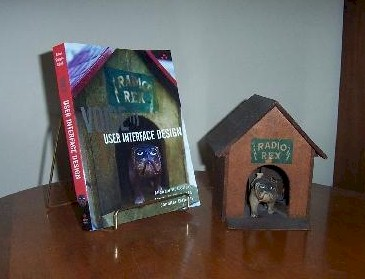
\includegraphics[scale=0.5]{images/radio_rex.jpg}
  \caption{雷克斯玩具狗} \label{fig:radio_rex}
\end{figure}
這種玩具狗在1920年代被銷售販賣,
它的賣點是,
如果有人叫他的名字「雷克斯」(Rex)的時候,
他會從底座的彈簧上彈起來。
其原理是,
玩具狗的內部有安裝一個彈簧,
這彈簧被設計成只會被500赫茲(Hz)的聲音能量驅動,
而500赫茲大約是他的英文名字Rex中第一個共振峰的頻率。

在1940年代以前,
語音辨識頂多就是像雷克斯玩具狗的共振峰辨識器一樣,
功能非常有限。
直到1940年代晚期,
才開始有一些自動化語音辨識系統被實做出來。
這邊舉兩個代表性的例子:
首先,
貝爾實驗室(Bell Lab)做了一個單一語者,可以辨識10個數字的系統。
他們的作法是在系統中存了單一語者對應十個數字的十種樣式(Patterns),
在辨識的時候就分別搜尋十種樣式,
傳回對應最高相關係數(Correlation Coefficient)的那個數字。
這樣做就可以讓系統正確率達到97\%到99\%。
第二,
在倫敦則有另一組人馬做了一個音素辨識器(Phoneme Recognizer),
它們除了採用跟前者類似的技術辨識四個母音與九個子音之外,
還率先提出音素轉移機率(Phoneme Transition Probability)的概念,
並用在他們的音素辨識器中好提昇辨識率,

到了1960年代晚期,
也是語音辨識技術革新的時期,
多數的語音辨識的技術面臨換血。
這邊列舉三個方面:

首先,
一些嶄新的抽取特徵演算法(Feature Extraction Algorithms)被提出。
包括快速傅立葉轉換(Fast Fourier Transform; FFT)、
在倒頻譜(Cepstral)空間裡處理語音訊號、
以及使用線性預測編碼(Linear Prediction Coding; LPC)來做語音編碼(Speech Coding)。

第二,
新的扭曲(Warping)技術出現。
所謂的扭曲即對訊號做時間偏移、伸展來解決說話速度(Speaking Rate)不一或訊號長度不同等問題。
扭曲一般來講都是用動態規劃(Dynamic Programming)來解決,
只是輸入的特徵向量不同而已。
舉例來講,
在早期線性預測編碼都只有用來做語音編碼。
但板倉氏結合了動態規劃的技巧與線性預測編碼。
他先對輸入的語音抽取線性預測編碼作為特徵向量,
然後對特徵向量做動態規劃來進行比對(Match)。

第三,
隱藏式馬可夫模型被應用到語音上。
隱藏式馬可夫模型是在1966年由統計學家波氏(Baum)提出\cite{BaumHMM}。
五年後,
由兩個實驗室獨立地將隱藏式馬可夫模型套用在語音上。
一個是當時在卡內基美隆(Carnegie Mellon University)唸書的貝克氏(Baker),
在讀了波式的隱藏式馬可夫模型的論文後,
將演算法應用到語音處理上。
另一個則是當時在IBM瓦特森實驗室(Watson Lab)的詹氏(Frederick Jelinek),
受到夏農(Shannon)的消息理論(Information Theory)影響而發展出跟隱藏式馬可夫模型等價的系統。
IBM的系統跟Baker的系統基本上一樣,
唯獨解碼演算法(Decoding Algorithm)不同。
Baker的系統使用維特比(Viterbi)解碼演算法,
而IBM則使用堆疊(Stack)解碼演算法。

之後的20年,
由於美國國防部陸續生出了許多語音辨識方面的計畫。
像是Resource Management, Wall Street Journal Air Traffic Information System, Broadcast News, CALLHOME等等。
藉由這些計畫的交流
隱藏式馬可夫模型也因此在研究社群中廣泛地被接受。
也因為它簡潔有效率,又有高正確率的優點,
至今仍鮮有方法可以撼動它的地位。

從以上簡述的歷史可以知道,
隱藏式馬可夫模型極其重要。
因此,
以下將簡述現今被普遍使用在語音辨識的貝氏定理架構,
隱藏式馬可夫模型便是建築在此架構上。
下一章我們再詳細說明隱藏式馬可夫模型。

如果我們把語音辨識想做是給定一串訊號,
找出一個句子它唸起來最像這串訊號。
在機率模型的架構下我們可以用條件機率來表示。
假設$x$是給定的觀測語句(Observation),
也就是處理訊號過後產生的特徵向量序列(Feature Vector Sequence),
$X$是所有可能的觀測語句。
則要從所有文句$Y$中找出機率最大的文句$y^{*}$可表示成
\begin{equation}
  y^{*} = \arg \max_{y \in Y} P(y | x)
\end{equation}
其中$y$為所有文句$Y$中的某一句,
$P(y | x)$代表在$x$發生時,文句$y$的事後機率。

剩下的問題就是,
我們要如何對$P(Y | X)$建立機率模型。
以上說起來很簡單,
但實際上由於語音辨識本身的複雜度,
對於$P(Y | X)$直接建立模型是有困難度的。
於是我們就用貝氏定理(Bayes Theorem)來轉換建模方向。
\begin{equation}
  \begin{split}
    y^{*} 
    &= \arg \max_{y \in Y} P(y | x) \\
    &= \arg \max_{y \in Y} \frac{ P(x | y) P(y) }{ P(x) } \\
  \end{split}
\end{equation}
由於我們在辨識的時候都是一句一句,
所以分母的$P(x)$在辨識一個句子的時候並不重要,
因此可以重寫成:
\begin{equation}
  \begin{split}
    y^{*} 
    &= \arg \max_{y \in Y} P(y | x) \\
    &= \arg \max_{y \in Y} P(x | y) P(y) \\
  \end{split}
\end{equation}
因此,
語音辨識的問題便被拆成如何替$P(X | Y)$及$P(Y)$建立模型。
其中$P(X | Y)$可以看作是,
給定一個句子的情況下,
唸出來的訊號是$X$的機率分佈。
而$P(Y)$則可以看成,
出現句子$Y$的機率分佈。
它們對應的稱呼便是聲學模型(Acoustic Model)及語言模型(Language Model),
也符合它們實際的意義。。

如研究動機一節所述,
本論文不沿用隱藏式馬可夫模型所使用的貝氏機率架構。
而是直接替$P(Y|X)$建立模型。
為了簡化起見,
$Y$只建立到音素辨識一層而非語言辨識一層。
而作為基礎實驗的隱藏式馬可夫模型,
也就沒有使用語言模型的分數,
而是做無設限之音素辨識(Free-Phone Decoding)。

\section{相關研究}
  語音辨識的聲學模型這一塊,
  現今大多數研究傾向在隱藏式馬可夫模型為主體的架構下抽換掉某些模型元件(Component),
  試試看辨識結果是否會進步。
  包括更換掉作為隱藏式馬可夫模型輸入的特徵
  (如使用類神經網路輸出的音框上音素的事後機率\cite{HermanskyTandem}、
  使用條件隨機域輸出的音框上音素的事後機率\cite{FoslerCrandem}),
  或更改目標函數(最小分類錯誤估測法\cite{Juang}、最小音素錯誤模型訓練法\cite{Povey})等。

  但最近這幾年仍有嘗試直接去為$P(Y|X)$建立模型的研究,
  像是隱藏式條件隨機域(Hidden Conditional Random Field; HCRF) \cite{AlexHCRF, SungHCRF},
  或是條件隨機域使用多層感知器(Multi-Layered Perceptron; MLP)的事後機率當作輸入\cite{MorrisCRF}等等。
  
  至於本論文使用的結構化支撐向量機(Structural Support Vector Machine)\cite{SVMstruct}的相關研究,
  有本論文主要依據的用結構化支撐向量機來做標籤序列(Sequence  Tagging)\cite{Altun03hiddenmarkov},
  (這也是結構化支撐向量機模型剛發展時率先的應用)
  也有將結構化支撐向量機拿來作資訊檢索\cite{JoachimsSVMperf, YisongSVMMAP}。
  由於結構化支撐向量機模型參數最佳化的困難,
  也有提出更好的最佳化演算法的論文\cite{JoachimsLinearSVM}。
  甚至有研究者注意到條件隨機域與結構化支撐向量機模型結構的相似性,
  寫了技術論文比較條件隨機域與結構化支撐向量機\cite{CRFvsSVMstruct} 。
  語音方面則還沒有人探討如何應用。

\section{本論文主要的研究方法及成果}
  本論文主要探討結構化支撐向量機學習演算法是否適合拿來解決語音辨識這個問題。
  由於模型結構的複雜性,
  先嘗試使用TIMIT這套語料來做問題相對單純的音素辨識。
  實驗結果發現,
  結構化支撐向量機學習演算法在直接使用傳統特徵向量像是梅爾倒頻譜係數(Mel-Frequency Cepstral Coefficient; MFCC)、
  感知線性預測係數(Perceptron Linear Prediction; PLP)時效果不太好,
  但如果仿照串接式系統(Tandem)的模式,
  先利用多層感知器將特徵向量轉換成音素在音框上的事後機率(Posterior Probability),
  再餵進結構化支撐向量機學習演算法的時候,
  絕對的辨識正確率卻可以贏過串接式系統約1\%。

\section{章節安排}
  本論文第二章將介紹基礎實驗中使用的隱藏式馬可夫聲學模型,以及串接式系統。
  第三章將介紹支撐向量機,
  由於結構化支撐向量機的概念是基於支撐向量機,
  全面了解支撐向量機演算法的話對於理解結構化支撐向量機十分有幫助。
  所以第三章從支撐向量機設計的理念到最佳化(Optimization)演算法給予完整的推導。
  第四章將介紹結構化支撐向量機,
  介紹該模型不同於其他模型的關鍵,
  並說明用來估測結構化支撐向量機模型參數的逼近演算法。
  第五章將介紹實驗環境、
  完整的實驗流程及結果呈現並進行分析。
  第六章會提出總結以及未來展望。

\chapter{背景知識}
  本章將介紹論文中作為基礎實驗的隱藏式馬可夫模型及串接式系統(Tandem)。
由於語音辨識中所使用的隱藏式馬可夫模型是連續分佈隱藏式馬可夫模型(Continuous Hidden Markov Model; Continuous-HMM),
所以這章介紹的是連續分佈隱藏式馬可夫模型而非離散分佈隱藏式馬可夫模型(Discrete Hidden Markov Model; Discrete-HMM)。
在本章中段則介紹多層感知器的理論,
這是因為串接式系統會使用到多層感知器(Multi-Layered Perceptron; MLP)。
最後,
我們介紹串接式系統的架構。

\section{連續分佈隱藏式馬可夫模型}
  隱藏式馬可夫模型(Hidden Markov Model, HMM)被廣泛地應用於不同問題,
  現今只要是問題跟序列標籤(Sequence Tagging)或是序列分段(Seqeunce Segmentation)相關的問題,
  都有隱藏式馬可夫模型的蹤影,
  像是詞類標籤(Part-of-speech Tagging)、統計語言模型(Statistical Language Modeling)等屬於自然語言處理(Natural Language Processing; NLP)的問題。
  跟語音辨識不同的是,
  在自然語言處理的問題中,
  特徵向量多半是離散(Discrete)的,
  即特徵向量空間(Feature Vector Space)是有限可數的(Finitely Countable)。
  因此,
  隱藏式馬可夫模型中每一個狀態(State)的放射機率(Emission Probability)分佈可以用機率質量函數(Probability Mass Function)來表示,
  這種隱藏式馬可夫模型我們稱作離散分佈隱藏式馬可夫模型(Discrete Hidden Markove Model)。
  語音辨識中的特徵向量每一維則都是實數,
  也就是說特徵向量空間是不可數的(Uncountable),
  所以必須把放射機率分佈改成為機率密度函數(Probability Density Function)才能正常運作。
  由於語音辨識使用的是連續分佈隱藏式馬可夫模型,
  以下我們將用數學的語言描述它的結構、參數估測的演算法。
  
  \subsection{模型結構}
    隱藏式馬可夫模型屬於統計模型中的生成模型(Generative Model),
    這表示我們假設要建立模型的對象是經由一連串丟骰子的動作而得到的。
    \begin{algorithm} 
      \begin{algorithmic}[1]
	\STATE 上帝依照它自己的意思,創造出$M$個狀態:$\mathbf{\Omega} = \lbrace 1, 2, \ldots M\rbrace$。大自然的運行就只是在這幾個狀態間跳來跳去
	\STATE 上帝丟一顆遵守均勻分佈(Uniform Distribution)的骰子$\mathbf{\pi}$,骰子的每一面代表$M$種狀態中的一個狀態,來決定大自然一開始在哪個狀態。
	\STATE 上帝創造出一顆特別的骰子$\mathbf{A}$,骰子的每一面也是$M$個狀態中的一種,但丟出哪一面的機率是依據之前丟出的$l$種狀態是什麼。
	\STATE 上帝再創造另一顆特別的骰子$\mathbf{B}$,骰子的每一面是人類實際觀察到諸多現象的一種,這諸多現象有可能是有限可數(Finitly Countable)、無限可數(Infinitly Countable)或不可數(Uncountable)。出現哪一種現象的機率是依據現在大自然處在什麼樣的狀態。
	\FOR{$t = 1, \dots, T$}
	  \STATE 上帝丟骰子$\mathbf{A}$,來決定大自然下一個狀態是什麼狀態。 
	  \STATE 進入下一個狀態後,上帝丟骰子$\mathbf{B}$來決定人類看到的是什麼現象。
	\ENDFOR
      \end{algorithmic}
      \caption{上帝的演算法} 
      \label{alg:god}
    \end{algorithm}
    今天我們觀察到一個序列,
    我們假設這個序列是(哲學上的)上帝是經由演算法\ref{alg:god}來產生的,
    也就是我們看到的一連串現象都是由大自然對應的一系列狀態來產生。
    其中骰子$\mathbf{A}$, $\mathbf{B}$, $\mathbf{\pi}$在這裡都假設是已知。
    則我們可以用有限狀態機(Finite State Machine; FSM)來表示上帝的演算法,
    每個圓圈代表演算法中的狀態,
    而邊(Edge)則表示轉移機率。
    如圖\ref{fig:general_hmm}所示。
    (為了容易表示,這邊假設骰子$\mathbf{B}$可以表達成機率質量函數,並且假設$l = 1$)。
    \begin{figure}
      \begin{center}
	\begin{tikzpicture}[->,>=stealth',shorten >=1pt,auto,node distance=5cm,semithick]
	\tikzstyle{every state}=[fill=white,draw=black,text=black]

	\node[state]	       (A)                    {};
	\node[state]	       (B) [below left of=A]  {};
	\node[state]	       (C) [below right of=A] {};

	\path (A) edge [bend right]  node {0.1}		(B)
		  edge [bend left] node {0.2}		(C)
		  edge [loop above] node {0.7}		()
	      (B) edge [bend left] node {0.4}		(C)
		  edge [bend right] node {0.05}		(A)
		  edge [loop left]  node {0.55}		()
	      (C) edge [bend left]  node {0.3}		(A)
		  edge [bend left] node {0.3}		(B)
		  edge [loop right] node {0.4}		();
	\end{tikzpicture}
      \end{center}
      \caption{隱藏式馬可夫模型}
      \label{fig:general_hmm}
    \end{figure}

    我們下列來說明隱藏式馬可夫模型所有的參數。
    在說明之前,
    先來定義符號。
    我們用$\mathbf{X}_t$表示第$t$個時間時產生現象的隨機變數、
    而$s_t$則表示在第$t$個時間狀態的隨機變數。
    \begin{itemize}
      \item $l$:轉移到下一個狀態的機率是根據之前$l$個的狀態來決定,
	所以要將隱藏式馬可夫模型描述完整的話,
	要說成$l$階隱藏式馬可夫模型($l$-th-order Hidden Markov Model; $l$-th-order HMM),
	一般來說,
	在語音辨識或自然語言處理的問題中,
	我們用的都是一階隱藏式馬可夫模型。
	本論文從這邊開始,
	我們沒有特別說明的話,
	提及隱藏式馬可夫模型都是指一階隱藏式馬可夫模型(First-order Hidden Markov Model; First-order HMM)。

      \item $\mathbf{\Omega} = \lbrace 1, 2, \ldots, M\rbrace$:
	表示隱藏式馬可夫模型的狀態字典集(Alphabet Set)。
	同時也包含進了有限狀態機總共有$M$個狀態這項參數,
	其編號從$1$到$M$。

      \item $\mathbf{O}_W$: 
	為隱藏式馬可夫模型的現象字典集(Observation Alphabet Set)。
	這個字典集可能是有限可數(Finitly Countable)、無限可數(Infinitely Countable)、不可數(Uncountable)。
	其中不可數的現象字典集我們必須使用連續分佈隱藏式馬可夫模型才能為現象建立模型。

      \item $\mathbf{A} = \lbrace a_{ij} \rbrace$:
	即上帝演算法中的骰子$\mathbf{A}$。
	表示從給定前$l$個狀態轉移到下一個狀態的轉移機率(Transition Probability)。
	如果是一階隱藏式馬可夫模型的話,
	$\mathbf{A}$就是一個二維的矩陣(Matrix),
	其中$a_{ij}$代表由前一個狀態$i$,
	轉移到下一個狀態$j$的機率。
	即
	\begin{equation}
	  a_{ij} = P(s_t = j | s_{t-1} = i)
	\end{equation}

      \item $\mathbf{B} = \lbrace b_j(\mathbf{x}) \rbrace$:
	即上帝演算法中的骰子$\mathbf{B}$。
	代表如果現在的狀態是狀態$j$,
	產生的現象(Observation)為$\mathbf{x}$的機率,
	我們稱為放射機率(Emission Probability)。
	即
	\begin{equation}
	  b_j(\mathbf{x}) = P(X_t = \mathbf{x} | s_t = j)
	\end{equation}
	如果放射機率是機率質量函數的話,
	我們可以進一步將上式寫成
	\begin{equation}
	  b_j(o_k) = P(X_t = o_k | s_t = j)
	\end{equation}
	其中$o_k$代表現象字典集中的第$k$個字符。
	於是$\mathbf{B}$就可以表示成: (狀態數)$\times$(現象字典集大小)的一個二維矩陣。

	但假如放射機率是機率密度函數的話,
	我們就必須假設某個機率分佈家族(Probability Distribution Family)。
	一般來說,
	我們都是假設多變量混合高斯密度函數(Multivariate Gaussian Mixture Density Function)來做為我們的機率密度函數。
	它的好處是,
	只要混合數的數量足夠多,
	他就可以逼近任何連續的機率密度函數。
	所以我們假設我們有$C$個高斯密度函數
	則放射機率可以寫成下列式子:
	\begin{equation}
	  b_j(\mathbf{x}) = \sum_{k=1}^C c_{jk} N(\mathbf{x}, \mu_{jk}, \Sigma_{jk}) = \sum_{k=1}^C c_{jk} b_{jk}(\mathbf{x}) 
	\end{equation}
	其中$b_{jk}(\mathbf{x}) = N(\mathbf{x}, \mu_{jk}, \Sigma_{jk})$代表的是
	附屬於第$j$個狀態、
	平均值(Mean)向量為$\mu_{jk}$、
	共變異(Covariance)矩陣為$\Sigma_{jk}$的一個高斯密度函數,
	而$c_{jk}$是每一個元件(Component)的權重,
	必須滿足加起來為1的條件。
	\begin{equation}
	  \sum_{k=1}^C c_{jk} = 1
	\end{equation}

      \item $\mathbf{\pi} = \lbrace \pi_i \rbrace$:
	這邊的$\mathbf{\pi}$就是上帝的骰子$\mathbf{\pi}$。
	代表我們一開始從第$i$個狀態開始的機率,
	又稱為初始機率(Initial Probability)。
	可以寫成有$M$個元素一維矩陣。
    \end{itemize}

    有上述的說明,
    很明顯隱藏式馬可夫模型的參數有一些限制如下:
    \begin{align}
      &a_{ij} \geq 0, b_i(\mathbf{x}) \geq 0, \pi_i \geq 0, \forall i, j, k \\
      &\sum_{j=1}^M a_{ij} = 1	\\
      &\int_{x \in \mathbf{O}_W} b_i(\mathbf{x}) = 1 \\
      &\sum_{i=1}^M \pi_i = 1 
    \end{align}

    儘管一階隱藏式馬可夫模型可以是任意有限狀態機的形式,
    但對於序列標籤或序列分段的問題,
    我們一般是假設有限狀態機的結構是從左到右,
    即只有轉移到右邊的狀態或轉移到自己的時候轉移機率才不為零。
    其結構如圖\ref{fig:left_to_right_hmm}
    \begin{figure}
      \begin{center}
	\begin{tikzpicture}[->,>=stealth',shorten >=1pt,auto,node distance=2.8cm,semithick]
	\tikzstyle{every state}=[fill=white,draw=black,text=black]

	\node[state]	       (A)                    {1};
	\node[state]	       (B) [right of=A]	      {2};
	\node[state]	       (C) [right of=B]	      {3};
	\node[state]	       (D) [right of=C]       {4};
	\node[state]           (E) [right of=D]       {5};

	\path (A) edge              node {1.0} (B)
	      (B) edge		    node {0.4} (C)
		  edge [loop above] node {0.6} ()
	      (C) edge              node {0.5} (D)
		  edge [loop above] node {0.5} ()
	      (D) edge              node {0.1} (E)
		  edge [loop above] node {0.9} ();
	\end{tikzpicture} 
      \end{center}
      \caption{從左到右的隱藏式馬可夫模型}
      \label{fig:left_to_right_hmm}
    \end{figure}

    到目前為止,
    我們都是假設隱藏式馬可夫模型的參數是已知的,
    下一節,
    我們將說明如何從訓練語料集估測隱藏式馬可夫模型的參數。
    為了數學式子寫起來簡潔,
    我們定義:
    \begin{equation}
      \Phi = (\mathbf{A}, \mathbf{B}, \mathbf{\pi}) 
    \end{equation}
    這樣我們再寫模型參數的時候只要寫一個$\Phi$就行了,
    而不用將$\mathbf{A}, \mathbf{B}, \mathbf{\pi}$都寫出來。

  \subsection{模型參數估測}
    首先我們假設訓練語料集(Training Set)$Z$由從1開始編號的$N$個樣本點所組成,
    數學定義如下:
    \begin{equation}
	Z = \lbrace X^{(n)} \rbrace_{n=1}^{N}
    \end{equation}
    其中每個樣本點又代表一個特徵向量序列(Feature Vector Sequence),
    $(\mathbf{X}_i^{(n)})$表示第$n$個樣本點的第$i$個特徵向量。

    我們這邊用最大相似度估測法(Maximum Likelihood Estimation)來估測參數,
    首先$N$個樣本點的相似度(Likelihood)可以寫成下式:
    \begin{equation}
      \prod_{n=1}^N P(X^{(n)}; \Phi)
    \end{equation}
    對相似度取對數可以幫助我們運算,
    於是對數相似度(Log-Likelihood)如下:
    \begin{equation}
      l(\Phi) = \sum_{n=1}^N \log P(X^{(n)} ; \Phi)
    \end{equation}

    我們希望將連續式隱藏式馬可夫模型的參數調適(Fit)到訓練語料集,
    但由於連續式隱藏式馬可夫模型的狀態是隱藏變數(Hidden Variable),
    所以直接用最大相似度估測法有困難,
    我們改用期望值最大法(Expectation Maximization)來估測參數。
    首先,
    將對數相似度重寫如下:
    \begin{equation}
      \begin{split}
	l(\Phi) 
	&= \sum_{n=1}^N \log P(X^{(n)} ; \Phi) \\
	&= \sum_{n=1}^N \log \left( \sum_{S^{(n)}} P(X^{(n)}, S^{(n)}; \Phi) \right) \\
	&= \sum_{n=1}^N \log \left( \sum_{S^{(n)}} \sum_{K^{(n)}} P(X^{(n)}, S^{(n)}, K^{(n)}; \Phi) \right) \\
      \end{split}
    \end{equation}

    接著,
    按照期望值最大法,
    我們假設$Q_n(S^{(n)}, K^{(n)})$是某個機率分佈,
    其中$S^{(n)}$是代表狀態序列(State Sequence)的隱藏變數,
    $K^{(n)}$則代表混合高斯模型中所使用的第幾個高斯密度函數所形成序列的隱藏變數。
    因此我們有
    \begin{align}
      &\sum_{S^{(n)}} \sum_{K^{(n)}} Q_n(S^{(n)}, K^{(n)}) = 1 \\
      &Q_n(S^{(n)}, K^{(n)}) \geq 0
    \end{align}
    根據詹氏不等式(Jensen's Inequality),
    推導對數相似度的下限(Lower Bound):
    \begin{equation}
      \begin{split}
	l(\Phi) 
	&= \sum_{n=1}^N \log \left( \sum_{S^{(n)}} \sum_{K^{(n)}} P(X^{(n)}, S^{(n)}, K^{(n)}; \Phi) \right) \\
	&= \sum_{n=1}^N \log \left( \sum_{S^{(n)}} \sum_{K^{(n)}} Q_n(S^{(n)}, K^{(n)}) \frac{P(X^{(n)}, S^{(n)}, K^{(n)}; \Phi)}{Q_n(S^{(n)}, K^{(n)})} \right) \\
	&\geq \sum_{n=1}^N \sum_{S^{(n)}} \sum_{K^{(n)}} Q_n(S^{(n)}, K^{(n)}) \log \left( \frac{P(X^{(n)}, S^{(n)}, K^{(n)}; \Phi)}{Q_n(S^{(n)}, K^{(n)})} \right) \\
	&= \sum_{n=1}^N \sum_{S^{(n)}} \sum_{K^{(n)}} Q_n(S^{(n)}, K^{(n)}) \log \left( P(X^{(n)}, S^{(n)}, K^{(n)}; \Phi) \right) \\
	&- \sum_{n=1}^N \sum_{S^{(n)}} \sum_{K^{(n)}} Q_n(S^{(n)}, K^{(n)}) \log \left( Q_n(S^{(n)}, K^{(n)}) \right) 
	\label{eq:jensen_lower_bound}
      \end{split}
    \end{equation}
    為了要讓下限盡量緊一些,
    讓詹式不等式的等號成立是最好。
    這表示必須讓隨機變數等於某個常數的機率為1。
    如下:
    \begin{equation}
	\frac{P(X^{(n)}, S^{(n)}, K^{(n)}; \Phi)}{Q_n(S^{(n)}, K^{(n)})} = c
    \end{equation}
    所以
    \begin{equation}
	P(X^{(n)}, S^{(n)}, K^{(n)}; \Phi) \propto Q_n(S^{(n)}, K^{(n)})
    \end{equation}
    再加上$\sum_{S^{(n)}} \sum_{K^{(n)}} Q_n(S^{(n)}, K^{(n)}) = 1$的限制,
    因此
    \begin{equation}
      \begin{split}
	Q_n(S^{(n)}, K^{(n)})
	&= \frac{P(X^{(n)}, S^{(n)}, K^{(n)}; \Phi)}{\sum_{S^{(n)}} \sum_{K^{(n)}} P(X^{(n)}, S^{(n)}, K^{(n)}; \Phi)} \\
	&= \frac{P(X^{(n)}, S^{(n)}, K^{(n)}; \Phi)}{P(X^{(n)}; \Phi)} \\
	&= P(S^{(n)}, K^{(n)} | X^{(n)}; \Phi) 
      \end{split}
    \end{equation}
    所以我們知道,
    當$Q_n(S^{(n)}, K^{(n)}) = P(S^{(n)}, K^{(n)} | X^{(n)}; \Phi)$時下限是最緊的。

    注意到式子\ref{eq:jensen_lower_bound}中後面一項在一個循環之中是不變的。
    \begin{equation}
      \sum_{n=1}^N \sum_{S^{(n)}} \sum_{K^{(n)}} Q_n(S^{(n)}, K^{(n)}) \log \left( Q_n(S^{(n)}, K^{(n)}) \right) 
    \end{equation}
    所以我們只需要最大化
    \begin{equation}
      \sum_{n=1}^N \sum_{S^{(n)}} \sum_{K^{(n)}} Q_n(S^{(n)}, K^{(n)}) \log \left( P(X^{(n)}, S^{(n)}, K^{(n)}; \hat{\Phi}) \right) \\ 
    \end{equation}
    其中,
    為了避免混淆(我們接下來要做最大化,只有原始的機率分佈參數需要變動),
    我們這邊在$P(X^{(n)}, S^{(n)}, K^{(n)}; \hat{\Phi})$用$\hat{\Phi}$來代替$\Phi$。

    我們將取期望值步驟中得到的$Q_i$代入:
    \begin{equation}
      \begin{split}
	&\sum_{n=1}^N \sum_{S^{(n)}} \sum_{K^{(n)}} Q_n(S^{(n)}, K^{(n)}) \log \left( P(X^{(n)}, S^{(n)}, K^{(n)}; \hat{\Phi}) \right) \\
	&= \sum_{n=1}^N \sum_{S^{(n)}} \sum_{K^{(n)}} \frac{P(X^{(n)}, S^{(n)}, K^{(n)}; \Phi)}{P(X^{(n)}; \Phi)} \log \left( P(X^{(n)}, S^{(n)}, K^{(n)}; \hat{\Phi}) \right) 
      \end{split}
    \end{equation}
    由於我們假設的是有限狀態機的結構,
    因此$P(X^{(n)}, S^{(n)}, K^{(n)} | \hat{\Phi})$可以寫成:
    \begin{equation}
      \begin{split}
	P(X^{(n)}, S^{(n)}, K^{(n)} | \hat{\Phi}) 
	&= \prod_{t=1}^T \hat{a}_{s_{t-1} s_t} \hat{b}_{s_t} (X^{(n)}_{t})\\
	&= \prod_{t=1}^T \hat{a}_{s_{t-1} s_t} \hat{b}_{s_t k_t} (X^{(n)}_{s_t}) \hat{c}_{s_t k_t} 
      \end{split}
    \end{equation}
    對上式取對數,
    得到
    \begin{equation}
     \log P(X^{(n)}, S^{(n)}, K^{(n)} | \hat{\Phi}) = \sum_{t=1}^T \log \hat{a}_{s_{t-1} s_t} + \sum_{t=1}^T \log \hat{b}_{s_t k_t} (x_t) + \sum_{t=1}^T \log \hat{c}_{s_t k_t}
    \end{equation}
    取對數後能夠拆解這項性質扮演了關鍵角色,
    這代表式子\ref{eq:jensen_lower_bound}也可以拆解。
    \begin{equation}
      \begin{split}
	&\sum_{n=1}^N \sum_{S^{(n)}} \sum_{K^{(n)}} P(S^{(n)}, K^{(n)} | X^{(n)}; \Phi) \log P(X^{(n)}, S^{(n)}, K^{(n)} | \hat{\Phi}) \\
	&= \sum_{n=1}^N \sum_{i=1}^{M} \sum_{j=1}^{M} \sum_{t=1}^T P(s_{t-1} = i, s_t = j | X^{(n)}; \Phi) \log \hat{a}_{ij} \\
	&+ \sum_{n=1}^N \sum_{j=1}^M \sum_{k=1}^C \sum_{t=1}^T P(s_t = j, k_t = k | X^{(n)}; \Phi) \log \hat{b}_{jk} (x^{(n)}_t) \\
	&+ \sum_{n=1}^N \sum_{j=1}^M \sum_{k=1}^C \sum_{t=1}^T P(s_t = j, k_t = k | X^{(n)}; \Phi) \log \hat{c}_{jk} \\
      \end{split}
    \end{equation}
    上面的式子可拆解代表我們做微分等於零的動作來最大化的時候,
    可以分別對每一項做最大化。
    更重要的是,
    第一項跟第三項的形式都是
    \begin{equation}
      F(x) = \sum_i y_i \log x_i
    \end{equation}
    且$\sum_i x_i = 1$。

    這種形式用拉氏乘數法(Lagrange Multiplier)就可以知道解是
    \begin{equation}
      x_i = \frac{y_i}{\sum_i y_i}
    \end{equation}
    因此第一項跟第三項的解分別為
    \begin{align}
      \hat{a}_{ij} = \frac{ \sum_{n=1}^N \sum_{t=1}^T \gamma^{(n)}_t (i,j) }{ \sum_{k=1}^M \sum_{n=1}^N \sum_{t=1}^T \gamma^{(n)}_t (i,j) } \\
      \hat{c}_{jk} = \frac{ \sum_{n=1}^N \sum_{t=1}^T \xi^{(n)}_t (j,k) }{ \sum_{k=1}^C \sum_{n=1}^N \sum_{t=1}^T \xi^{(n)}_t (j,k) }	  
    \end{align}
    其中$\xi^{(n)}_t (j, k)$代表
    \begin{equation}
      \xi^{(n)}_t (j, k) = P(s_t = j, k_t = k | X^{(n)}; \Phi)	
    \end{equation}  
    而$\gamma^{(n)}_t (i, j)$代表
    \begin{equation}
      \gamma^{(n)}_t (i, j) = P(s_{t-1} = i, s_t = j | X^{(n)}; \Phi)
    \end{equation}
    唯一比較複雜的是第二項,
    因為它又依賴於$\lbrace \mu_{jk}, \Sigma_{jk} \rbrace$。
    因此在做拉式乘數法的時候必須要使用鏈鎖法則(Chain Rule)。
    經過一連串運算,
    我們可以得到
    \begin{equation}
      \begin{split}
	\hat{\mu}_{jk} 
	&= \frac{ \sum_{t=1}^T P(s_t = j, k_t = k | X^{(n)} ;\Phi) x_t }{ \sum_{t=1}^T P(s_t = j, k_t = k | X^{(n)}; \Phi)} \\ 
	&= \frac{ \sum_{t=1}^T \xi^{(n)}_t(j, k) x_t }{ \sum_{t=1}^T \xi^{(n)}_t (j, k) } \\
      \end{split}
    \end{equation}

    \begin{equation}
      \begin{split}
	\hat{\Sigma}_{jk} 
	&= \frac{ \sum_{t=1}^T P(s_t = j, k_t = k | X^{(n)}; \Phi) (x_t - \hat{\mu}_{jk})(x_t - \hat{\mu}_{jk})^T }{ \sum_{t=1}^T P(s_t = j, k_t = k | X^{(n)}; \Phi) } \\
	&= \frac{ \sum_{t=1}^T \xi^{(n)}_t (j,k) (x_t - \hat{\mu}_{jk})(x_t - \hat{\mu}_{jk})^T }{ \sum_{t=1}^T \xi^{(n)}_t (j,k) } \\
      \end{split}
    \end{equation}

    \begin{algorithm}
      \caption{前向演算法(Forward Algorithm)}
      \label{alg:forward}
      \begin{algorithmic}[1]
	\FOR{$i = 1, \dots M$}
	  \STATE $\alpha_1(i) = \pi_i b_i(X_1)$ 
	\ENDFOR
	\FOR{$t = 2, \dots, T$}
	  \FOR{$i = 1, \dots, M$}
	    \STATE $\alpha_t(j) = \left[ \sum_{i=1}^M \alpha_{t-1}(i) a_{ij} \right] b_j(X_t)$ 
	  \ENDFOR
	\ENDFOR
	\STATE $P(X; \Phi) = \sum_{i=1}^M \alpha_T(i)$
      \end{algorithmic}
    \end{algorithm}
   
    現在最大的問題是,
    我們如何能夠將$\xi^{(n)}_t (j, k)$和$\gamma^{(n)}_t (i, j)$算出來。
    這就是波氏-維氏演算法(Baum-Welch Algorithm)發揮用處的地方。
    波氏-維氏演算法由演算法\ref{alg:forward}及演算法\ref{alg:backward}所構成。
    其中前向演算法(演算法\ref{alg:forward}可以幫助我們出$\alpha_t(i)$,
    代表的意思是
    \begin{equation}
      \alpha_t(i) = P(X_{1}^{t} | s_t = i; \Phi)
    \end{equation}
    而後向演算法(演算法\ref{alg:backward}可以幫助我們算出$\beta_t(i)$,
    代表的意思是
    \begin{equation}
      \beta_t(i) = P(X_{t+1}^T | s_t = i; \Phi)
    \end{equation}
    有了$\alpha_t(i)$跟$\beta_t(i)$, 
    我們就可以用下列式子算出$\xi^{(n)}_t (j, k)$和$\gamma^{(n)}_t (i, j)$。
    \begin{align}
      & \gamma^{(n)}_t (i, j) = \frac{ \sum_{k=1}^C \alpha_{t-1} (i) a_{ij} c_{jk} b_{jk} (x_t) \beta_t(j) }{ \sum_{i=1}^M \alpha_T(i) } \\ 
      & \xi^{(n)}_t (j, k) = \frac{ \sum_{i=1}^M \alpha_{t-1} (i) a_{ij} c_{jk} b_{jk} (x_t) \beta_t(j) }{ \sum_{i=1}^M \alpha_T(i) }  
    \end{align}
    將$\xi^{(n)}_t (j, k)$和$\gamma^{(n)}_t (i, j)$代入之前更新參數的式子,
    便可以得到新的一組參數。
    \begin{algorithm}
      \caption{後向演算法(Backward Algorithm)}
      \label{alg:backward}
      \begin{algorithmic}[1]
	\STATE $\beta_T(i) = \frac{1}{M}$ 
	\FOR{$t = T-1, \dots, 1$}
	  \FOR{$i = 1, \dots, M$}
	    \STATE $\beta_t(i) = \left[ \sum_{j=1}^M a_{ij} b_j(X_{t+1}) \beta_{t+1}(j) \right]$
	  \ENDFOR
	\ENDFOR
      \end{algorithmic}
    \end{algorithm}

\section{多層感知器(Multi-Layered Perceptron)}
  早期機器學習的研究者們受到神經科學(Neuro Science)的啟發,
  試著建立一個模型來模仿神經元突觸的行為。
  如圖\ref{fig:neuron},
  一個神經元的作用就是將它接受到的訊號,
  經過某種轉換後,
  再傳給下一個神經元。
  \begin{figure}
    \centering
    \subfloat[人體的神經元]{\label{fig:neuron}\includegraphics[scale=1.0]{images/neuron.pdf}}
    \subfloat[數學的神經元]{\label{fig:artificial_neuron}\includegraphics[scale=2.0]{images/math_neuron.pdf}}
  \end{figure}
  這跟數學上的函數其實是一樣的,
  因此我們只要想辦法找出一個函數符合真實神經元的情況也許就可以模擬其行為。
  但實際上我們並不知道那是什麼樣的函數。
  只好假設它是輸入向量線性組合的某個轉換,
  寫成數學式子如下:
  \begin{equation}
    F(\mathbf{x}) = \varphi \left( \sum_i w_i x_i \right)
  \end{equation}
  其中$\mathbf{x}$是輸入訊號,$\varphi$是某個數學轉換(Transformation),而$w_i$是線性組合的加權(Weight)。
  如果將上面的概念畫成圖,就像圖\ref{fig:artificial_neuron}一般。
  很明顯這樣的結構太簡單,
  無法提供我們強而有力的模型。
  但我們可以將這些小的神經元串接起來來得到一個強力的模型。
  而這樣串接起來的模型我們稱作類神經網路(Neuro Network)。
  但如果串接的結構太複雜,
  又超出我們可以計算的能力。
  所以我們限制其串接的結構,
  規定串接的時候只能串接成一個無迴路(Acyclic)的類神經網路,
  並給予它另一個名稱,
  叫做多層感知器(Multi-Layered Perceptron),
  又名前向遞推類神經網路(Feed-Forward Neural Network),
  為類神經網路的一個子集。
  其結構如圖\ref{fig:mlp}。
  經常的用途是對付分類(Classification)問題、迴歸(Regression)問題,或將高維的特徵向量轉換到較低維度的向量。
  \def\layersep{2.5cm}
  \begin{figure}
    \begin{center}
      \begin{tikzpicture}[shorten >=1pt,->,draw=black!50, node distance=\layersep]
	  \tikzstyle{every pin edge}=[<-,shorten <=1pt]
	  \tikzstyle{neuron}=[circle,fill=black!25,minimum size=17pt,inner sep=0pt]
	  \tikzstyle{input neuron}=[neuron, fill=green!50];
	  \tikzstyle{output neuron}=[neuron, fill=red!50];
	  \tikzstyle{hidden neuron}=[neuron, fill=blue!50];
	  \tikzstyle{annot} = [text width=4em, text centered]

	  % Draw the input layer nodes
	  \foreach \name / \y in {1,...,4}
	  % This is the same as writing \foreach \name / \y in {1/1,2/2,3/3,4/4}
	      \node[input neuron, pin=left:Input \#\y] (I-\name) at (0,-\y) {};

	  % Draw the hidden layer nodes
	  \foreach \name / \y in {1,...,5}
	      \path[yshift=0.5cm]
		  node[hidden neuron] (H-\name) at (\layersep,-\y cm) {};

	  % Draw the output layer node
	  \node[output neuron,pin={[pin edge={->}]right:Output}, right of=H-3] (O) {};

	  % Connect every node in the input layer with every node in the
	  % hidden layer.
	  \foreach \source in {1,...,4}
	      \foreach \dest in {1,...,5}
		  \path (I-\source) edge (H-\dest);

	  % Connect every node in the hidden layer with the output layer
	  \foreach \source in {1,...,5}
	      \path (H-\source) edge (O);

	  % Annotate the layers
	  \node[annot,above of=H-1, node distance=1cm] (hl) {Hidden layer};
	  \node[annot,left of=hl] {Input layer};
	  \node[annot,right of=hl] {Output layer};
      \end{tikzpicture}
    \end{center}
    \caption{多層感知器}
    \label{fig:mlp}
  \end{figure}

  一般來講,
  如果是在解二元分類問題(Binary Classification)或是單元迴歸問題(Univariate Regression)的時候,
  我們設定輸出的向量就是一維的實數向量。
  如果是分類問題就取一個門檻(Threshold),
  高過門檻就是某一個分類,
  低於門檻就是另一個分類。
  如果是迴歸問題就直接使用這個實數當作我們的預測值。

  當解的問題改成多元分類問題或多元迴歸問題時,
  我們可以增加輸出向量的維數為要分類的類別數來解決問題,
  而用來估測模型參數的演算法並不會需要更動。
  
  以下,
  我們用數學的語言來描述多層感知器模型。
  
  \subsection{數學定義}
  為了方便說明模型的架構,
  這邊假設我們希望建立模型的函數是$f: \mathbb{R}^d \rightarrow \mathbb{R}$,
  即輸入的向量為$d$維,輸出的向量是一維。
  而我們建立模型的函數為$g$,
  我們希望$g$跟$f$越相近越好。

  則我們定義我們的前向遞推類神經網路如下:
  網路由$L$層串接起來的神經元(Neuron)們所組成,
  第$l$($1 \leq l \leq L$)層總共有$d^{(l)}$個神經元,
  將$d^{(l-1)}$個輸入接成$d^{(l)}$個輸出,
  這樣的結構表示第$l-1$層的輸出就是第$l$層的輸入。
  (注意如果是有跳層情況的網路,也可以重新寫成第$l$層的輸入從第$l-1$層輸出來的形式,
  所以定義由無迴路性質刻畫是正確的)。
  由以上定義,
  我們知道整個系統的輸入維度為$d^{(0)} = d$,
  而整個系統的輸出維度為$d^{(L)} = 1$。

  接著,
  我們再定義第$l$層的輸入為$x_i^{(l-1)}, (1 \leq i \leq d^{(l-1)})$、
  輸出為$x_j^{(l)}, (1 \leq j \leq d^{(l)})$。
  而第$l$層的加法權重為$w_{ij}^{(l)}, (1 \leq l \leq L, 0 \leq i \leq d^{(l-1)}, 1 \leq j \leq d^{(l)})$
  則第$l$層中的第$j$個神經元的轉換函數可定義為
  \begin{equation}
    x_j^{(l)} = \varphi \left( \sum_{i=0}^{d^{(l-1)}} w_{ij}^{(l)} x_i^{(l-1)} \right)
  \end{equation}
  其中$\varphi(s) = \tanh(s) = \frac{e^s - e^{-s}}{e^s + e^{-s}}$。

  為了後面演算法的推導方便,
  我們定義一個輔助變數$s_j^{(l)}$將神經元函數中線性的部份跟非線性的部份分開來。
  \begin{align}
    &s_j^{(l)} = \sum_{i=0}^{d^{(l-1)}} w_{ij}^{(l)} x_i^{(l-1)} \\
    &x_j^{(l)} = \varphi(s_j^{(l)})
  \end{align}
  假設模型的參數為已知,
  則使用類神經網路來計算函數$g(\mathbf{x})$的預測值便可以如下操作:
  將輸入向量$\mathbf{x}$的每一維分別擺到$x_1^{(0)}, \ldots x_{d^(0)}^{(0)}$,
  再從第一層開始一一按照上面的神經元函數計算這一層的輸出,
  直到第$L$層為止。
  則最後我們便將$x_1^{(L)}$當作$g(\mathbf{x})$輸出的值。

  \subsection{模型參數估測}
  有了前一節定義的多層感知器結構,
  這一節將探討如何利用訓練集$Z = \lbrace (\mathbf{x}_n, y_n) \rbrace_{n=1}^{N}$,
  來估計多層感知器模型的參數。

  為了要衡量我們得到的參數究竟讓模型是否更貼近我們希望建立模型的函數,
  我們需要一個錯誤衡量函數(Error Function)。
  一般來講,
  在訓練多層感知器的錯誤衡量函數都是
  \begin{equation}
    E_n(w) = (g(\mathbf{x}_n) - y_n)^2
  \end{equation}
  用二次項的好處就是可以微分,
  方便我們使用做最佳化(Optimization)的時候使用梯度下降法(Gradient Decent)。

  在這邊我們使用一種在實做上比較容易的一種梯度下降法 -- 隨機梯度下降法(Stochastic Gradient Decent)來做最佳化,
  因此我們需要計算$\frac{\partial E_n}{\partial w_{ij}^{(l)}}, 0 \leq i \leq d^{(l-1)}, (1 \leq j \leq d^{(l)}, 1 \leq l \leq L)$。
  一旦我們有了以上梯度,
  則我們可以應用隨機梯度下降法來修正權重。
  \begin{equation}
    w_{ij}^{(l)} \leftarrow w_{ij}^{(l)} - \eta \frac{\partial E_n}{\partial w_{ij}^{(l)}}
  \end{equation}
  其中$\eta$是學習速率,
  隨機梯度下降法只要執行足夠多次更新,
  就可以得到一組滿意的參數。
  \begin{algorithm}
    \caption{隨機梯度下降演算法(Stochastic Gradient Decent Algorithm)}
    \label{alg:stochastic_gradient_decent}
    \begin{algorithmic}[1]
      \STATE 視問題將$w^{(0)}$初始化為0或一組亂數。
      \FOR{$t = 1, 2, \dots, T$}
	\STATE $w^{(t)} \leftarrow w^{(t-1)} - \eta \nabla E(w^{(t-1)})$
      \ENDFOR
    \end{algorithmic}
  \end{algorithm}
  所以主要的問題是,
  是否有方法讓我們可以快速地算出$\frac{\partial E_n}{\partial w_{ij}^{(l)}}$。
  這便是我們下面要講的後向推進演算法(Backpropagation Algorithm)的目的。

  假設我們已經執行了一遍前向遞推來計算出對應訓練範例的輸出,
  在這過程中,
  注意到輔助變數$x_j^{(l)}$跟$s_j^{(l)}$已經被計算出來。
  則由於$w_{ij}^{(l)}$只透過$s_j^{(l)}$來影響輸出,
  根據鏈鎖法則(Chain Rule),
  我們有
  \begin{equation}
    \frac{\partial E_n}{\partial w_{ij}^{(l)}} = \frac{\partial E_n}{\partial s_j^{(l)}} \times \frac{\partial s_j^{(l)}}{\partial w_{ij}^{(l)}}
  \end{equation}

  其中$\frac{\partial s_j^{(l)}}{\partial w_{ij}^{(l)}} = x_i^{(l-1)}$是已經計算出來的值。
  所以只剩下如何計算$\frac{\partial E_n}{\partial s_j^{(l)}}$的問題。
  先定義$\delta_j^{(l)} = \frac{\partial E_n}{\partial s_j^{(l)}}$。
  則在最後一層$l = L$的時候,
  我們有$E_n = (x_1^{(L)} - y)^2$,
  因此我們能計算$\delta_1^{(L)}$
  \begin{equation}
    \delta_1^{(L)} = \frac{\partial E_n}{\partial s_j^{(l)}} 
    = \frac{\partial E_n}{\partial x_1^{(l)}} \times \frac{\partial x_1^{(L)}}{\partial s_1^{(l)}}
  \end{equation}
  其中$\frac{\partial E_n}{\partial x_1^{(l)}} = 2(x_1^{(L)} - y)$、
  $\frac{\partial x_1^{(L)}}{\partial s_1^{(l)}} = \varphi^{'}(s_1^{(L)})$。
  因此我們有了遞迴的初始條件。
  我們可以利用遞迴來算第$l-1$的$\delta_j^{(l-1)}$
  \begin{equation}
    \begin{split}
      \delta_i^{(l-1)} 
      &= \frac{\partial E_n}{\partial s_i^{(l-1)}} \\
      &= \sum_{j=1}^{d^{(l)}} \frac{\partial E_n}{\partial s_j^{(l)}} \times 
      \frac{\partial s_j^{(l)}}{\partial x_i^{(l-1)}} \times
      \frac{\partial x_i^{(l-1)}}{\partial s_i^{(l-1)}} \\
      &= \sum_{j=1}^{d^{(l)}} \delta_j^{(l)} \times w_{ij}^{(l)} \times \varphi^{'}(s_i^{(l-1)})
    \end{split}
  \end{equation}
  其中$\varphi^{'}(s) = 1 - \varphi^2(s)$、
  $\varphi(s_i^{(l)}) = x_i^{(l)}$
  因此$\delta_i^{(l-1)}$可以遞迴地表示成如下:
  \begin{equation}
    \delta_i^{(l-1)} = \left( 1 - (x_i^{(l-1)})^2 \right) \sum_{j=1}^{d^{(l)}} w_{ij}^{(l)} \delta_j^{(l)}
  \end{equation}
  以上的式子中的變數都在前向遞推時能算出來,
  因此我們藉由後向推進演算法就可以算出所有的$\delta$。
  有了$\delta$,我們就可以算出錯誤對權重的梯度。
  因此,
  我們可以做隨機梯度下降法來最佳化。

\section{串接式聲學模型(Tandem)}
  \usetikzlibrary{calc,trees,positioning,arrows,chains,shapes.geometric,%
      decorations.pathreplacing,decorations.pathmorphing,shapes,%
      matrix,shapes.symbols}

  \tikzset{
  >=stealth',
    punktchain/.style={
      rectangle, 
      rounded corners, 
      % fill=black!10,
      draw=black, very thick,
      text width=10em, 
      minimum height=3em, 
      text centered, 
      on chain},
    line/.style={draw, thick, <-},
    element/.style={
      tape,
      top color=white,
      bottom color=blue!50!black!60!,
      minimum width=8em,
      draw=blue!40!black!90, very thick,
      text width=10em, 
      minimum height=3.5em, 
      text centered, 
      on chain},
    every join/.style={->, thick,shorten >=1pt},
    decoration={brace},
    tuborg/.style={decorate},
    tubnode/.style={midway, right=2pt},
  }

  \begin{figure}
    \begin{tikzpicture}
    [node distance=.8cm,
    start chain=going below,]
	\node (asym) [punktchain ]  {多層感知器};
	\begin{scope}[start branch=venstre,
	  %We need to redefine the join-style to have the -> turn out right
	  every join/.style={->, thick, shorten <=1pt}, ]
	  \node[punktchain, on chain=going left, join=by {<-}]
	      (risiko) {抽取特徵向量};
	\end{scope}
	\begin{scope}[start branch=abc,]
	\node (finans) [punktchain, on chain=going right, join=by {->}] {事後機率解碼器};
	\end{scope}
    \node[punktchain, join,] (kerker) {主成份分析法};
    \node[punktchain, join,] (disk) {隱藏式馬可夫程式集混合高斯模型};
    \node[punktchain, join,] (makro) {隱藏馬可夫程式集解碼器};
    % Now that we have finished the main figure let us add some "after-drawings"
    %% First, let us connect (finans) with (disk). We want it to have
    %% square corners.
    %\draw[|-,-|,->, thick,] (finans.south) |-+(0,-1em)-| (disk.north);
    \end{tikzpicture}
    \label{fig:tandem_flow_chart}
    \caption{串接式系統流程圖}
  \end{figure}
  串接式系統(Tandem)\cite{HermanskyTandem}整體的架構如圖\ref{fig:tandem_flow_chart}。
  如果瞭解原本隱藏式馬可夫模型的系統架構的話,
  串接式系統其實很容易瞭解。
  它等於是將原本餵進隱藏式馬可夫模型的特徵向量做過一次轉換,
  再當作另一種特徵向量餵進隱藏式馬可夫模型。
  而這種轉換就是用多層感知器加上主成分分析法(Pricipal Component Analysis; PCA)來達成。
  
  整體過程如下:
  首先先將原本用來訓練隱藏式馬可夫模型的訓練資料,
  對每個音框都標上對應正確的次字元標籤
  (一般來講,就是音素標籤),
  來作為訓練多層感知器的訓練資料集。
  而這裡多層式感知器的用途,
  是輸入一個音框及其鄰近音框,
  輸出這個音框屬於某個音素的事後機率。
  因此,
  多層感知器的輸入維度為特徵向量的維度乘上一個窗戶長
  (一般取現在這個音框加上前後四個音框,共九個音框),
  輸出維度為次字元標籤的數量,
  一般使用在串接式系統的多層感知器都是三層,
  扣掉第一層、第三層為輸入、輸出,
  真正決定多層感知器力量是第二層的神經元數量,
  在做串接式系統的時候多半取1000左右。

  有了音框上次字元(Subword)的事後機率,
  一種選擇是直接對這串事後機率向量做解碼,
  這樣的架構稱為混合式系統(Hybrid System)。
  但根據赫氏(Hermansky)所述\cite{HermanskyTandem},
  由於次字元的標籤數多半在30個到50個之間,
  也就是說多層感知器輸出的向量維度也跟原本的語音特徵向量維度差不多,
  這樣對辨識結果並沒有特別的好處。

  由於事後機率的分佈擁有非常偏斜(Skew)的特性,
  因此我們將事後機率再取上一個對數(Log),
  將他轉到另一個空間去。
  轉換之後的空間讓向量擁有一個性質,
  就是其中一維的值會特別大,
  其他維則非常小。

  回到我們一開始說的,
  這個取了對數後的事後機率,
  就是轉換過後的特徵向量,
  把它當作隱藏式馬可夫模型的輸入來訓練的話,
  根據文獻\cite{HermanskyTandem},
  便可以增進辨識率。
  如果在得到對數事後機率之後再做一次主成份分析降維,
  便可以再增進不少辨識,
  理由可能是這樣比較貼近於混合高斯密度函數的特性。

  至於在使用測試語料集(Testing Set)做辨識評估(Evaluation)的時候,
  便先利用由訓練集訓練的多層感知器將評估集的特徵向量轉換成對數事後機率。
  再餵進由對數事後機率訓練的隱藏式馬可夫模型,
  經由此模型來解碼出最有可能的路徑。

\section{本章總結}
  本章說明了作為本論文基礎實驗的隱藏式馬可夫模型以及串接式系統的理論基礎,
  並給出詳細的訓練演算法和流程。


\chapter{支撐向量機學習演算法}
  本章將介紹著名的支撐向量機(Support Vector Machine; SVM)學習演算法,
這邊的內容主要取材自\cite{VapnikSVM, Burges98tutorial}等論文。

\section{簡介}  
  當我們在考慮一個使用線性分類器(Linear Classifier)的二元分類問題(Binary Classification Problem)時
  (如圖\ref{fig:svm_intro_example}),
  我們很自然地會認為圖中的B點比起圖中的C點分對的機會要高,
  因為B點離分隔線(Seperating Line)的幾何距離(Geometric Distance)比起C點要來得大。
  同樣地,
  我們對A點分對的信心也比B點來得高。
  \begin{figure}  
    \begin{center}
      \begin{tikzpicture}[scale=1.5]
	  % Draw axes
	  \draw [<->,thick] (0,4) node (yaxis) [above] {$y$}
	      |- (5,0) node (xaxis) [right] {$x$};
	  % Draw two intersecting lines
	  \draw (0.5,4) coordinate (b_1) -- (5,0.5) coordinate (b_2);
	  % Calculate the intersection of the lines a_1 -- a_2 and b_1 -- b_2
	  % and store the coordinate in c.
	  \draw (3.7,4) node {A};
	  \draw (2.7,2.5) node {C};
	  \draw (1.7,3.8) node {B};
	  \fill[red] (2,3.8) circle (2pt);
	  \fill[red] (3,2.5) circle (2pt);
	  \fill[red] (4,4) circle (2pt);
	  \fill[blue] (1,0.6) circle (2pt);
	  \fill[blue] (4,1) circle (2pt);
	  \fill[blue] (2,0.4) circle (2pt);
      \end{tikzpicture}
    \end{center}
    \caption{使用線性分類器的二元分類問題} 
    \label{fig:svm_intro_example}
  \end{figure}      

  支撐向量機學習演算法(Support Vector Machine; SVM)的靈感即來自於二元分類問題中這「邊距」(Margin)的概念。
  既然一個點對分隔線的距離決定了我們對他分對的信心,
  那如果我們可以找到一個分隔線,
  使得其中一類跟另外一類間的邊距最大,
  這樣找到的分類線我們便對它最有信心。
  拿圖\ref{fig:svm_intro_example}中的二維平面範例來看的話,
  由於一條分隔線的參數是$(w, b)$
  (分隔線可以寫成$w_1 \cdot x_1 + b = 0$,
  或者是$\langle w, x \rangle + b$,
  其中$\langle \cdot, \cdot \rangle$代表內積),
  要讓邊距盡量大,
  就表示我們要決定一組$(w^{*}, b^{*})$,
  使得每一個紅色點代入$(w^{*}, b^{*})$時$\langle w^{*}, x \rangle + b^{*} \gg 0$,
  每一個藍色點代入$(w^{*}, b^{*})$時$\langle w^{*}, x \rangle + b^{*} \ll 0$。
  一旦決定了這組$(w^{*}, b^{*})$,
  有新的點進來的時候,
  我們只需要算出$\langle w^{*}, x \rangle + b^{*}$是大於0還是小於0,
  大於0的話就將它歸為一類、
  小於0就將它歸為另一類(等於0可以隨便指定一類)。
  即假設我們用支撐向量機學習演算法學得的函數是$f$,
  定義
  \begin{equation}
    sign(z) = 
    \left\{ 
      \begin{array}{l}
      1 \text{ if } z \geq 0 \\
      -1 \text{ otherwize } \\
      \end{array}
    \right.	
  \end{equation}
  則我們得到的分類器便是$sign(f(x))$

  同樣地道理,
  拓展到$n$維空間的時候,
  我們希望一個分隔超平面(Seperating Hyperplane)使得邊距最大。
  由這樣的原則所找到的分類器我們稱作極大邊距分類器(Maximum Margin Classifier)    

\section{原始形式(Primal Form)}
  在這一個章節我們將進行支撐向量機學習演算法理論的推導。
  為了讓推導容易理解,
  我們首先考慮樣本點是能用一個超平面(Hyperplane)完全正確地分隔開來(Seperable Case)的二元分類問題。
  說明這種情形之後,
  再推廣到容忍樣本點被分錯及非線性的情形。

  假設給定一組$N$點的訓練樣本集
  \begin{equation}
  Z = \lbrace (x_i, y_i) \rbrace_{i=1}^{N}
  \end{equation}
  其中$x_i \in \mathbb{R}^n$為特徵向量、$y_i \in \lbrace -1, 1 \rbrace$為標籤。
  為了符合我們找到讓邊距最大的超平面,
  好將正確樣本點與不正確樣本點盡可能分離的原則,
  我們直覺上來寫就是
  \begin{equation}
    \max_{w, b} \text{ Thickness}(w, b)
  \end{equation}
  其中Thickness為邊距的厚度,其是$w$和$b$的函數,
  
  但畢竟這不是數學的語言,
  我們需要更嚴謹的定義。
  首先我們定義
  \begin{equation}
    \rho_i = \left( \text{ distance of } x_i \text{ to } \langle w, x_i \rangle + b = 0 \right)
  \end{equation}
  用高中學過的幾何距離代入就變成下列式子
  \begin{equation}
    \rho_i = \left\vert \frac{ \langle w, x_i \rangle + b }{ \Vert w \Vert } \right\vert 
    = y_i \left( \frac{ \langle w, x_i \rangle + b }{ \Vert w \Vert } \right)
  \end{equation}    
  到這邊我們便可以將邊距定義成所有點中到超平面距離最小的幾何距離,
  寫成數學如下
  \begin{equation}
  \text{Thickness}(w, b) = \min_i \rho_i
  \end{equation}
  因此,
  要找到使邊距最厚的超平面,就代表我們要將上述最小的距離極大化。
  \begin{equation}
    \begin{split}
    &\max_{w, b} \min_i \rho_i, \\
    \text{s.t. } \forall i: &\rho_i = y_i \left( \frac{ \langle w, x_i \rangle + b }{ \Vert w \Vert } \right)
    \end{split}
  \end{equation}  
  但要處理這樣的問題不太容易,
  所以我們便將問題轉換一下,
  加入$\Vert w \Vert = 1$的限制,
  這樣便可以把$\Vert w \Vert$從限制條件的分母中拿掉
  (注意這邊只是加上$\Vert w \Vert = 1$,距離仍然算是幾何距離而非函數距離(functional distance))。
  \begin{equation}
    \begin{split}
      &\max_{w, b} \min_i \rho_i \\
      \text{s.t. } \forall i:  &\rho_i = y_n ( \langle w, x_i \rangle + b ), \\
      &\Vert w \Vert = 1
    \end{split}
  \end{equation}    
  我們定義$\rho = \min_i \rho_i$,
  由於$\rho$是最小的,所以我們有$\rho_i \geq \rho, \forall i$。
  則上述問題可以再寫成,
  \begin{equation}
    \begin{split}
      &\max_{w, b} \rho \\
      \text{s.t. } &\forall i: \rho_i \geq \rho, \\
      &\Vert w \Vert = 1
    \end{split}
  \end{equation}
  將$\rho_i$用$\langle w, x_i \rangle + b$代入
  \begin{equation} 
    \begin{split}
      &\max_{w, b} \rho \\
      \text{s.t. } \forall i: &y_i ( \langle w, x_i \rangle + b) \geq \rho, \\
      &\Vert w \Vert = 1 
    \end{split}
  \end{equation}        
  雖然我們前面將$\Vert w \Vert = 1$加入是為了消掉限制中分母的$\Vert w \Vert$,
  但基本上$\Vert w \Vert = 1$是個討厭的限制,
  它讓限制變成非凸的(non-convex),
  所以到這邊我們希望再把它拿掉,
  變成一個好解的形式。
  於是我們定義$\hat{\rho} = \Vert w \Vert \rho$並代入,
  則式子變成如下
  (這相當於把幾何距離的問題轉換成函數距離的問題。注意這邊的$\Vert w \Vert$不再等於1,所以$y_i ( \langle w, x_i \rangle + b)$其實是有擴大,相當於$\Vert w \Vert$倍)
  \begin{equation}
    \begin{split}
      &\max_{w, b: w \neq 0} \frac{\hat{\rho}}{\Vert w \Vert} \\
      \text{s.t. } \forall i: &y_i ( \langle w, x_i \rangle + b ) \geq \hat{\rho}
    \end{split}
  \end{equation}    
  雖然我們將$\Vert w \Vert = 1$從限制條件中拿掉使得限制不再是非凸的,
  但現在目標函數(Object Function)變成非凸的。
  而且解必定有無限多種,
  因為當一個最佳解$(w^{*}, b^{*})$存在的時候,
  則對任意$c$,$(cw^{*}, c b^{*})$亦同樣是最佳解。

  不過幸好,這些不等式的兩邊都是可以隨意擴大縮小的,    
  我們只要加回一個限制,
  即$\hat{\rho} = 1$,
  問題就得以解決,
  變成下列的形式
  \begin{equation}
    \begin{split}
      &\max_{w, b} \frac{\hat{\rho}}{\Vert w \Vert} \\
      \text{s.t. } \forall i: &y_i ( \langle w, x_i \rangle + b ) \geq \hat{\rho}, \\
      &\hat{\rho} = 1
    \end{split}
  \end{equation}    
  再整理一下,就變成 
  \begin{equation}
    \begin{split}
      &\max_{w, b} \frac{ 1 }{\Vert w \Vert} \\
      \text{s.t. } \forall i: &y_i ( \langle w, x_i \rangle + b ) \geq 1
    \end{split}
  \end{equation}  
  由於最大化$\frac{ 1 }{\Vert w \Vert}$等價於最小化$\Vert w \Vert$,
  但$\Vert w \Vert$這個目標函數並不容易最小化,
  我們可以用等價的二次式來取代,
  即$\Vert w \Vert^2$。
  另外,由於我們做最佳化時會對目標函數微分,
  也就是二次方會被打下來,所以我們前面多乘一個$\frac{1}{2}$好讓我們的微分式的係數變成1,
  變成下列式子
  \begin{equation}
    \begin{split}
      &\min_{w, b} \frac{1}{2} \Vert w \Vert^2  \\
      \text{s.t. } \forall i: &y_i ( \langle w, x_i \rangle + b ) \geq 1
    \end{split}
  \end{equation}   
  這便是一般最常見到的支撐向量機的核心公式,
  也是支撐向量機演算法的原始形式(Primal Form)。
  這個問題到這邊已經被我們轉換成由一個凸性的二次目標函數及許多線性的限制條件所構成的最佳化問題。
  實際上,
  這是一個二次規劃(Quadratic Programming)的問題,
  存在有效率的演算法。
  我們可以直接將上面的問題用任何解二次規劃的程式去解決。  
  不過,
  我們並不滿足於此,
  原始形式並不是支撐向量機演算法真正有威力的形式。
  我們接下來先介紹拉氏對偶性(Lagrange Duality),
  好將原始形式轉換成支撐向量機演算法的對偶形式(Dual Form)。
  對偶形式允許使用核心映射來高效地處理高維空間。

\section{拉氏對偶性(Lagrange Duality)}
  首先我們先來回憶一下微積分課程中,
  教我們如何用拉氏乘數法(Lagrange Multiplier)來解決下面有$l$個限制條件的最佳化問題
  \begin{equation}
    \begin{split}
      &\min_w f(w) \\
      \text{s.t. } \forall i \in \lbrace 1, &\cdots, k \rbrace: g_i(w) \leq 0, \\
      \forall j \in \lbrace 1, &\cdots, l \rbrace: h_i(w) = 0
    \end{split}
  \end{equation}
  微積分課本教我們說,
  首先我們定義拉氏輔助函數(Lagrange Function)為
  \begin{equation}
    \mathcal{L}(w, \alpha, \beta) = f(w) + \sum_{i=1}^k \alpha_i g_i(w) + \sum_{i=1}^l \beta_i h_i(w)
  \end{equation}
  其中$\alpha_i$和$\beta_i$被稱作拉氏乘數(Lagrange Multiplier)。    
  接著,	
  我們取拉氏輔助函數的偏導數為0來得到一組方程
  \begin{align}
    \frac{\partial \mathcal{L}}{\partial w_i} = 0 \\
    \frac{\partial \mathcal{L}}{\partial \beta_i} = 0 \\
    \frac{\partial \mathcal{L}}{\partial \alpha_i} = 0
  \end{align}
  解上面的方程而得到一組或多組駐點(Stationary Point)($w$,$\beta$)。
  在目標函數非凸的情況下,
  還要檢查這些駐點究竟是不是極值點。

  在定義對偶形式之前,
  就像推導二次規劃問題時一樣,
  我們必須先定義原始形式(Primal Form)。
  考慮下面函數$\theta_{\mathcal{P}}(w)$
  \begin{equation}
    \theta_{\mathcal{P}}(w) = \max_{\alpha, \beta: \alpha_i \geq 0} \mathcal{L}(w, \alpha, \beta)
  \end{equation}    
  我們定義原始形式為最小化$\theta_{\mathcal{P}}$
  即
  \begin{equation}
    \min_w \theta_{\mathcal{P}}(w)
  \end{equation}
  這看起來有點奇怪,
  甚至我們會懷疑這是否還等價於原本的問題
  但我們這樣定義為了造出對偶形式(最大化最小化順序相反)。

  首先我們要說明的是,
  先前的問題跟這邊的原始形式(Primal Form)是等價的。
  假如我們選定的某個$w$違反了某個原始形式中的限制條件,
  即存在$i$使得$g_i(w) > 0$或$h_i(w) \neq 0$,
  由於$\alpha_i$跟$\beta_i$能夠被調整成任意實數,
  最大化就相當於將$\alpha_i$或$\beta_i$取無限大而得到無限大。
  所以
  \begin{equation}
    \begin{split}
      \theta_{\mathcal{P}}(w) 
      & = \max_{\alpha, \beta, \alpha_i \geq 0} \mathcal{L}(w, \alpha, \beta) \\
      & = \max_{\alpha, \beta, \alpha_i \geq 0} \left( f(w) + \sum_{i=1}^k \alpha_i g_i(w) + \sum_{i=1}^l \beta_i h_i(w) \right) \\
      & = \infty
    \end{split}
  \end{equation}    
  相反地,
  如果給定的$w$滿足所有條件限制,
  則跟原本的$f$沒有兩樣。
  按照上面的分析,
  原始形式可以寫成如下
  \begin{equation}
    \theta_{\mathcal{P}}(w) =
    \left\{ 
      \begin{array}{l}
	f(w) \text{ if } w \text{ satisfies primal constraints } \\
	\infty \text{ otherwize } \\
      \end{array}
    \right.	
  \end{equation}
  因此我們可以知道,
  如果所有限制條件都被滿足,
  則$\theta_{\mathcal{P}}$的最小值跟$f$的最小值是一樣的。
  如果違反限制條件,
  則兩個的最小值都會取到正無限大。    
  因此原始形式是跟先前的問題等價的,
  並擁有相同的解。
  即
  \begin{equation}
    \min_w \theta_{\mathcal{P}}(w) = \min_w \max_{\alpha, \beta: \alpha_i \geq 0} \mathcal{L}(w, \alpha, \beta)    
  \end{equation}
  為了後面說明方便,
  我們假設原始形式的最佳解為
  \begin{equation}
    p^{*} = \min_w \theta_{\mathcal{P}}(w)
  \end{equation}    

  有了原始形式後,
  我們來看問題的對偶形式(Dual Form),
  並說明在什麼情況下對偶形式跟原始形式有相同的解。

  考慮下面函數
  \begin{equation}
    \theta_{\mathcal{D}}(\alpha, \beta) = \min_w \mathcal{L}(w, \alpha, \beta)    
  \end{equation}    
  跟之前的$\theta_{\mathcal{P}}$差別在他是對$w$做最小化。
  我們定義對偶形式如下
  \begin{equation}
    \max_{\alpha, \beta: \alpha_i \geq 0} \theta_{\mathcal{D}}(\alpha, \beta) = \max_{\alpha, \beta: \alpha_i \geq 0} \min_w \mathcal{L}(w, \alpha, \beta)    
  \end{equation}    
  可以看到,
  對偶形式跟原始形式的差別只在於最大化跟最小化的順序是相反的。
  我們假設對偶形式的最佳解為
  \begin{equation}
    d^{*} = \max_{\alpha, \beta: \alpha_i \geq 0} \theta_{\mathcal{D}}(w)
  \end{equation}    
  則很明顯地,
  原始形式跟對偶形式有如下的關係
  \begin{equation}
    d^{*} = \max_{\alpha, \beta: \alpha_i \geq 0} \min_w \mathcal{L}(w, \alpha, \beta) \leq \min_w \max_{\alpha, \beta: \alpha_i \geq 0} \mathcal{L}(w, \alpha, \beta) = p^{*}
  \end{equation}

  實際上,
  在目標函數$f$跟不等限制條件$g_i$都是凸性函數(Convex),相等限制條件$h_i$是仿射函數(Affine),
  且假設不等限制條件$g_i$是有解的(Feasible)(存在$w$使得$\forall i: g_i(w) < 0$)
  的情況底下,
  $d^{*}$會等於$p^{*}$。
  即必定存在$w^{*}$、$\alpha^{*}$、$\beta^{*}$使得
  $w^{*}$是原始形式的解,
  $\alpha^{*}$、$\beta^{*}$是對偶形式的解。
  並且$p^{*} = d^{*} = \mathcal{L}(w^{*}, \alpha^{*}, \beta^{*})$

  上面說的$w^{*}, \alpha^{*}, \beta^{*}$其實會滿足所謂的卡氏條件(Karush-Kuhn-Tucker Condition; KKT Condition)
  \begin{align}
    \frac{\partial}{\partial w_i} \mathcal{L}(w^{*}, \alpha^{*}, \beta^{*}) = 0, 1 \leq i \leq n \\
    \frac{\partial}{\partial \beta_i} \mathcal{L}(w^{*}, \alpha^{*}, \beta^{*}) = 0, 1 \leq i \leq l\\
    \alpha_i^{*} g_i (w^{*}) = 0, 1 \leq i \leq k \label{kkt_complement}\\
    g_i(w^{*}) \leq 0, 1 \leq i \leq k \\
    \alpha^{*} \geq 0, 1 \leq i \leq k  
  \end{align}
  在目標函數非凸的時候,
  卡氏條件只是必要條件而已,
  但幸運的是,
  在支撐向量機中目標函數是凸性的,
  所以只要$w^{*}, \alpha^{*}, \beta^{*}$滿足卡氏條件,
  它就是原始形式及對偶形式的一組解。

  注意到卡氏條件中一條重要的式子(\ref{kkt_complement}),
  它又被稱作為卡氏對偶互補條件(KKT Dual Complementarity Condition)。
  (它隱含說假如$\alpha_i^{*} > 0$,則$g_i(w^{*}) = 0$,
  對於$\alpha_i^{*} > 0$這樣的條件我們稱為激發的(Active),
  因為它式子為等號而非不等號)。
  它之所以重要是因為在支撐向量機的推導過程中,
  顯示了相較於全部的樣本點,
  支撐向量(Support Vectors)的數量是非常少的。
  並且,
  我們也可以用它來測試最佳化的收斂程度。

\section{對偶形式}
  了解了拉氏對偶性後,
  我們再回來看原本的邊距分類器的問題。
  \begin{equation}
    \begin{split}
      &\min_{w, b} \frac{1}{2} \Vert w \Vert^2  \\
      \forall i: y_i &( \langle w, x_i \rangle + b \geq 1
    \end{split}
  \end{equation}
  首先我們把上述式子中的條件限制重寫成符合前一節$g_i(w)$的形式
  \begin{equation}
    g_i(w) = -y_i (\langle w, x_i \rangle + b) + 1 \leq 0
  \end{equation}
  接著我們可以寫出拉氏輔助函數
  \begin{equation}
    \mathcal{L}(w, b, \alpha) = \frac{1}{2} \Vert w \Vert^2 - \sum_{i=1}^N \alpha_i (y_i ( \langle w, x_i \rangle + b) - 1) \label{lagrangian} 
  \end{equation}
  注意這邊拉氏乘數只有$\alpha_i$而沒有$\beta_i$
  根據前一節的定義,
  原始形式為
  \begin{equation}
    \min_w \max_{\alpha, \beta: \alpha_i \geq 0} \mathcal{L}(w, b, \alpha)
  \end{equation}
  而對偶形式為
  \begin{equation}
    \max_{\alpha, \beta: \alpha_i \geq 0} \min_w \mathcal{L}(w, b, \alpha) 
  \end{equation}
  因此
  我們要先利用拉氏乘數法最小化$\mathcal{L}(w, b, \alpha)$。
  我們分別對$w$及$b$取偏導數為零。
  得到
  \begin{align}
    \nabla_w \mathcal{L}(w, b, \alpha) = w - \sum_{i=1}^N \alpha_i y_i x_i = 0 \label{partial_w}\\
    \frac{\partial}{\partial b} \mathcal{L}(w, b, \alpha) = \sum_{i=1}^N \alpha_i y^{(i)} = 0 \label{b_equal_0} 
  \end{align}
  根據式子(\ref{partial_w})可推出
  \begin{equation}
    w = \sum_{i=1}^N \alpha_i y_i x_i \label{sum_equal_w} 
  \end{equation}
  我們將式子(\ref{sum_equal_w})代回式子(\ref{lagrangian})可以得到
  \begin{equation}
    \mathcal{L}(w, b, \alpha) = \sum_{i=1}^N \alpha_i - \frac{1}{2} \sum_{i, j=1}^N y_i y_j \alpha_i \alpha_j x_i x_j - b \sum_{i=1}^N \alpha_i y_i   
  \end{equation}
  但根據式子(\ref{b_equal_0}),
  上式中最後一項是0
  所以我們得到
  \begin{equation}
    \mathcal{L}(w, b, \alpha) = \sum_{i=1}^N \alpha_i - \frac{1}{2} \sum_{i, j=1}^N y_i y_j \alpha_i \alpha_j x_i x_j    
  \end{equation}
  由於我們是調整$w$跟$b$來最小化$\mathcal{L}$而得到上式,
  所以跟之前的一些限制條件擺在一起就變成了支撐向量機的對偶形式
  \begin{equation}
    \begin{split}
    \max_{\alpha} W(\alpha) = &\sum_{i=1}^N \alpha_i - \frac{1}{2} \sum_{i, j=1} y_i y_j \alpha_i \alpha_j \langle x_i, x_j \rangle \\
      s.t. &\alpha_i \geq 0, \forall i \\
      &\sum_{i=1}^N \alpha_i y_i = 0 \\
    \end{split}
  \end{equation}
  而在支撐向量機的問題中,
  很明顯目標函數是凸性函數,
  且相等限制條件$h_i$是仿射函數,
  因此原始形式跟對偶形式有相同的解。
 
  在章節\ref{sec:SMO}中,
  我們將介紹解對偶形式的最佳化演算法。
  這邊我們先假設能解出$\alpha$,
  則我們可以利用式子(\ref{sum_equal_w})可以算出$w^{*}$,
  有了$w^{*}$,
  我可以用下列式子算出$b$
  \begin{equation}
    b^{*} = - \frac{ \max_{i:y_i = -1} w^{*T} x_i + \min_{i: y_i = 1} w^{*T} x_i }{ 2 }
  \end{equation}

  在我們進入下一節之前,
  我們來看一下卡氏對偶互補條件。
  從卡氏對偶互補條見我們得知只有滿足$y_i ( \langle w, x_i \rangle - \theta) = 1$
  (即函數邊距(Funtional Margin)剛好等於1)
  才會有$\alpha_i^{*} > 0$。
  這相當於圖\ref{fig:support_vectors}中那些落在虛線上的點。
  因此在圖中的情形就是只有對應虛線上三點的$\alpha_i$大於0。
  \begin{figure}
    \begin{center}
      \begin{tikzpicture}[scale=1.5]
	  % Draw axes
	  \draw [<->,thick] (0,5) node (yaxis) [above] {$y$}
	      |- (6,0) node (xaxis) [right] {$x$};
	  % Draw two intersecting lines
	  \draw (1,4) coordinate (b_1) -- (5,1) coordinate (b_2);
	  \draw[dashed] (1.5,4.5) coordinate (b_1) -- (5.5,1.5) coordinate (b_2);
	  \draw[dashed] (0.5,3.5) coordinate (b_1) -- (4.5,0.5) coordinate (b_2);
	  % Calculate the intersection of the lines a_1 -- a_2 and b_1 -- b_2
	  % and store the coordinate in c.
	  \fill[red] (4,2.625) circle (2pt);
	  \fill[red] (2.5,3.75) circle (2pt);
	  \fill[red] (4,4) circle (2pt);
	  \fill[blue] (2.5,2) circle (2pt);
	  \fill[blue] (4,0.5) circle (2pt);
	  \fill[blue] (2,0.4) circle (2pt);
      \end{tikzpicture}
    \end{center}
    \caption{支持向量}
    \label{fig:support_vectors}
  \end{figure}
  我們稱這些滿足$y_i ( \langle w, x_i \rangle - \theta) = 1$的點為支持向量(Support Vectors)

  在支撐向量機學習演算法裡面,
  這些$\alpha_i > 0$的點讓我們可以使用一些特別的技巧,
  像是我們要替一個特徵向量$x$分類的時候,
  我們把$x$代入$\langle w, x \rangle + b$中來看看值究竟是大於0或小於0。
  但$\langle w, x \rangle + b$又可以寫成
  \begin{equation}
    \begin{split}
      \langle w, x \rangle + b 
      &= \left\langle \sum_{i=1}^N \alpha_i y_i x_i, x \right\rangle + b \\
      &= \sum_{i=1}^N \alpha_i y_i \langle x_i, x \rangle + b \label{inner_product}
    \end{split}
  \end{equation}
  我們可以看到式子(\ref{inner_product})中,
  實際上要計算預測值都是靠那些$\alpha_i > 0$對應的$\langle x_i, x \rangle$,
  這樣看起來,
  我們做預設時都是在靠這些支撐著邊界的點,
  因此,
  我們的模型才叫支撐向量機。
  
\section{核心映射}
  在上一節之中,
  我們看到在算預測值的時候其實只要依靠與支持向量的內積就可以了
  \begin{equation}
    \langle w, x \rangle + b = \sum_{i=1}^N \alpha_i y_i \langle x_i, x \rangle + b \label{inner_product}
  \end{equation}
  這個性質可以讓我們玩一些小技巧。

  回想我們在做分類或回歸問題時,
  如果輸入的特徵向量是$x$,
  我們常常會多加一些額外經過轉換的特徵,
  譬如$x^2$、$x^3$等試試看是否對問題有正面的幫助,
  這相當於把原本的內積$\langle x, z \rangle$換成特徵向量某個映射後的內積$\langle \phi(x), \phi(z) \rangle$。
  這樣加上額外特徵的壞處就是會增加向量維度,
  兩個向量內積所花費的時間也就增加了。
  
  但換個角度想,
  假如適當選取上述的$\phi$,
  則$\langle \phi(x), \phi(z) \rangle$其實是可能很輕鬆算出來的。
  於是我們只要直接算
  \begin{equation}
    K(x, z) = \langle \phi(x), \phi(z) \rangle
  \end{equation}
  就好了。

  舉例來說,
  假設$x, z \in \mathfrak{R}^n$,
  考慮
  \begin{equation}
    K(x, z) = (x^T z)^2
  \end{equation}
  這個$K(x, z)$整理後可以寫成兩個向量的內積
  \begin{equation}
    \begin{split}
      K(x, z) 
      & = \left( \sum_{i=1}^n x_i z_i \right) \left( \sum_{j=1}^n x_i z_i \right) \\
      & = \sum_{i=1}^n \sum_{j=1}^n x_i x_j z_i z_j \\
      & = \sum_{i, j=1}^n (x_i x_j) (z_i z_j) \\
    \end{split}
  \end{equation}
  因此,
  假設$n = 3$,
  則特徵映射$\phi$為
  \begin{equation}
    \phi(x) =    	
    \left[ 
    x_1 x_1, 
      x_1 x_2,
      x_1 x_3,
      x_2 x_1,
      x_2 x_2,
      x_2 x_3,
      x_3 x_1,
      x_3 x_2,
      x_3 x_3
    \right]^T
  \end{equation}
  儘管計算出$\phi(x)$再做內積需要$O(n^2)$的時間,
  但計算$K(x,z)$只要$O(n)$的時間就可以了。

\section{不可分的情形}
  前面的章節我們都假設資料是可分的(Separable),
  儘管做了核心映射會增加資料可分的可能性,
  但我們不能被保證每次碰到的資料都是可分的。
  就算是可分的,
  也可能因為離群值(Outlier)而找到沒那麼理想的超平面。
  如圖\ref{fig:outlier}
  \begin{figure}
    \begin{center}
      \subfloat{
      \begin{tikzpicture}[scale=1]
	  % Draw axes
	  \draw [<->,thick] (0,5) node (yaxis) [above] {$y$}
	      |- (6,0) node (xaxis) [right] {$x$};
	  % Draw two intersecting lines
	  \draw (0.5,4.375) coordinate (b_1) -- (5.5,0.625) coordinate (b_2);
	  % Calculate the intersection of the lines a_1 -- a_2 and b_1 -- b_2
	  % and store the coordinate in c.
	  \fill[red] (4,2.625) circle (2pt);
	  \fill[red] (2.5,3.75) circle (2pt);
	  \fill[red] (4,4) circle (2pt);
	  \fill[blue] (2.5,2) circle (2pt);
	  \fill[blue] (4,0.5) circle (2pt);
	  \fill[blue] (2,0.4) circle (2pt);
      \end{tikzpicture}}
      \subfloat{
      \begin{tikzpicture}[scale=1]
	  % Draw axes
	  \draw [<->,thick] (0,5) node (yaxis) [above] {$y$}
	      |- (6,0) node (xaxis) [right] {$x$};
	  % Draw two intersecting lines
	  \draw (1,5) coordinate (b_1) -- (5,0.5) coordinate (b_2);
	  % Calculate the intersection of the lines a_1 -- a_2 and b_1 -- b_2
	  % and store the coordinate in c.
	  \fill[red] (4,2.625) circle (2pt);
	  \fill[red] (2.5,3.75) circle (2pt);
	  \fill[red] (4,4) circle (2pt);
	  \fill[blue] (0.5,5) circle (2pt);
	  \fill[blue] (2.5,2) circle (2pt);
	  \fill[blue] (4,0.5) circle (2pt);
	  \fill[blue] (2,0.4) circle (2pt);
      \end{tikzpicture}}
    \end{center}
    \caption{支持向量}
    \label{fig:outlier}
  \end{figure}
  我們採用$L_1$規範化($L_1$ Regularization)的方式來重寫我們的原始形式(Primal Form),
  引進鬆弛變數(Slack Variable)$\xi_i$到原本的支撐向量機的限制及目標函數中,
  \begin{equation}
    \begin{split}
      &\min_{w,b} \frac{1}{2} \Vert w \Vert^2 + C \sum_{i=1}^N \xi_i \\
      \text{s.t.} y_i &(\langle w, x_i \rangle + b) \geq 1 - \xi_i \\
      &\xi_i \geq 0
    \end{split}
  \end{equation}
  這種寫法讓函數邊距(Functional Margin)有可能小於1,
  但如果一個函數邊距為$1 - \xi_i$,
  則我們在目標函數必須付出$C \xi_i$的代價。
  這邊的$C$在讓邊距變小以及多半資料點的函數邊距至少為1兩個目標之間做取捨。

  要得到對偶形式,
  一樣我們要先定義拉氏輔助函數
  \begin{equation}
    \mathcal{L}(w, b, \xi, \alpha, r) = \frac{1}{2} \langle w, w \rangle + C \sum_{i=1}^N \xi_i - \sum_{i=1}^N \alpha_i [y_i (\langle w, x \rangle + b) - 1 + \xi_i ] - \sum_{i=1}^N r_i \xi_i
  \end{equation}
  其中$\alpha_i$跟$r_i$是拉氏乘數。
  經過類似之前的討論之後,
  我們便可以得到對偶形式。
  唯一要注意的是卡氏對偶互補條件改變成
  \begin{align}
    \alpha_i = 0 \Rightarrow y_i (\langle w, x_i \rangle + b) \geq 1 \\
    \alpha_i = C \Rightarrow y_i (\langle w, x_i \rangle + b) \leq 1 \\
    0 < \alpha_i < C \Rightarrow y_i (\langle w, x_i \rangle + b) = 1
  \end{align}
  加入$L_1$規範化後的對偶形式如下
  \begin{equation}
    \begin{split}
      \max_{\alpha} W(\alpha) = &\sum_{i=1}^N \alpha_i - \frac{1}{2} \sum_{i,j=1}^N y_i y_j \alpha_i \alpha_j \langle x_i, x_j \rangle \\
      \text{s.t.} &0 \leq \alpha_i \leq C \\
      &\sum_{i=1}^N \alpha_i y_i = 0
    \end{split}
  \end{equation}
  令人意外的是,
  儘管加入$L_1$規範化,
  對偶形式只有從限制$\alpha_i \geq 0$,
  改變成$0 \leq \alpha_i \leq C$。
  至於如何解對偶形式,
  跟之前可分的情形一樣,
  都是依靠下一節介紹的循序最小化方法。

\section{循序最小化方法(Sequential Minimal Optimization)} \label{sec:SMO}
  循序最小化方法(Sequential Minimal Optimization; SMO)是由普拉特氏(Platt)在1998年提出\cite{Microsoft98SMO},
  用來解決支撐向量機的對偶形式。
  為什麼要從對偶形式下手?
  前面的章節已經提出幾個對偶形式的優點,
  像是可以使用核心映射。
  除此之外,
  算支撐向量機的參數相當於是解一個非常龐大的二次規劃(Quadratic Programming)。
  如果我們無法拆解這個龐大的二次規劃問題,
  那我們就無法拓展到比較大的訓練集,
  而對偶形式有一些好的性質讓我們能夠把這個龐大的二次規劃拆成比較小的二次規劃,
  再用分析的方法解這些比較小的二次規劃。

  循序最小化方法就是這樣的一個方法,
  不僅可以將原本龐大的問題拆解,
  概念上也比較簡單(亦即程式比較好寫)。
  循序最小化方法概念上其實很像梯度下降法(Gradient Decent),
  只是一次要更新兩個變數而非一個。
  回想支撐向量機的式子,
  \begin{equation}
    \begin{split}
      \max_{\alpha} W(\alpha) = &\sum_{i=1}^N \alpha_i - \frac{1}{2} \sum_{i,j=1}^N y_i y_j \alpha_i \alpha_j \langle x_i, x_j \rangle \\
      \text{s.t. } &\forall k, 0 \leq \alpha_k \leq C \\
      &\sum_{k=1}^N \alpha_k y_k = 0
    \end{split}
  \end{equation}
  如果我們有一組滿足限制的$\alpha_i$,
  我們不可能只變動$\alpha_i$而固定其他的$\alpha_j$,
  這是因為
  \begin{equation}
    \begin{split}
      & \sum_{k=1}^N \alpha_k y_k = 0 \label{eq:sum_to_zero} \\
      & \Rightarrow \alpha_i y_i = - \sum_{j \neq i} \alpha_j y_j
    \end{split}
  \end{equation}
  也就是$\alpha_i$是被唯一決定的。

  因此我們必須一次挑選兩個變數,
  整個循序最小化方法看起來會如演算法\ref{alg:over_simplified_smo},
  \begin{algorithm}
    \caption{循序最小化方法}
    \label{alg:over_simplified_smo}
    \begin{algorithmic}[1]
      \REPEAT
	\STATE 使用啟發子(Heuristic)來選取$\alpha_i$跟$\alpha_j$,這兩個$\alpha$會讓更新的差盡量大
	\STATE 固定其他$\alpha$、調整$\alpha_i$跟$\alpha_j$來讓$W(\alpha)$最大化
      \UNTIL{收斂}
    \end{algorithmic}
  \end{algorithm}
  其中測試收斂是用卡氏條件是否都在邊界值加上某個誤差$tol$內。

  剩下的問題是,
  我們選好$\alpha_i$跟$\alpha_j$後要怎麼固定其他$\alpha$來最大化$W(\alpha)$。
  不失一般性,
  這邊假設我們是要變動$\alpha_i$跟$\alpha_j$並固定剩下的$\alpha$。
  則根據式子(\ref{eq:sum_to_zero}),
  我們有
  \begin{equation}
    \alpha_i y_i + \alpha_j y_j = - \sum_{k \neq i, j} \alpha_k y_k
  \end{equation}
  由於右半邊是定值,
  我們可以寫成
  \begin{equation}
    \alpha_i y_i + \alpha_j y_j = \zeta
  \end{equation}
  其中$\zeta$為常數。

  由這個式子,
  我們可以畫出圖\ref{fig:smo_line_constraint}。
  \begin{figure}
    \begin{center}
      \begin{tikzpicture}[scale=1.2]
	  % Draw axes
	  \draw [<->,thick] (0,5) node (yaxis) [above] {$\alpha_1$}
	      |- (5,0) node (xaxis) [right] {$\alpha_2$};
	  % Draw two intersecting lines
	  \draw (0.5,0) coordinate (b_1) -- (4.5,4) coordinate (b_2);
	  \draw (0,4.5) coordinate (b_1) -- (4.5,4.5) coordinate (b_2);
	  \draw (4.5,4.5) coordinate (b_1) -- (4.5,0) coordinate (b_2);
	  \draw[dashed] (0,4) coordinate (b_1) -- (4.5,4) coordinate (b_2);
	  \draw (4,3.8) node {$\alpha_i y_i + \alpha_j y_j = \zeta$};
	  \draw (4.6, 0.1) node {$C$};
	  \draw (0.1, 4.6) node {$C$};
	  \draw (0.1, 4.1) node {$H$};
	  \draw (0.1, 0.13) node {$L$};
	  % Calculate the intersection of the lines a_1 -- a_2 and b_1 -- b_2
	  % and store the coordinate in c.
      \end{tikzpicture}
    \end{center}
    \caption{分析法}
    \label{fig:smo_line_constraint}
  \end{figure}
  明顯地,
  $\alpha_i$跟$\alpha_j$必定落在圖中的$[0, C] \times [0, C]$範圍中的$\alpha_i y_i + \alpha_j y_j = \zeta$那條線上。
  也就是說,
  $\alpha_j$一定落在圖中的$L$跟$H$之間($L \leq \alpha_j \leq H$)。
  不然$(\alpha_i, \alpha_j)$沒辦法同時滿足以上限制。
  要算出一般的$L$跟$H$如下
  \begin{itemize}
    \item If $y_i \neq y_j$, $L = \max(0, \alpha_j - \alpha_i), H = \min(C, C + \alpha_j - \alpha_i)$ 
    \item If $y_i = y_j$, $L = \max(0, \alpha_i + \alpha_j - C), H = \min(C, \alpha_i + \alpha_j)$
  \end{itemize}

  另外,由於$\alpha_i + \alpha_j = \zeta$,
  所以$\alpha_i$可以寫成$\alpha_j$的函數
  \begin{equation}
    \alpha_i = (\zeta - \alpha_j y_j) y_i
  \end{equation}
  也就是說$W(\alpha_i, \alpha_j, \mathbf{\alpha})$是$\alpha_j$的二次式
  \begin{equation}
    \begin{split}
      W(\alpha_i, \alpha_j, \mathbf{\alpha}) 
      = W((\zeta - \alpha_j y_j y_i), \alpha_j, \mathbf{\alpha})
      = a \alpha_j^2 + b \alpha_j + c
    \end{split}
  \end{equation}
  由於$W(\alpha_i, \alpha_j, \mathbf{\alpha})$是單變數的二次式,
  也就是凸性函數。
  因此,
  容易驗證如果求出的最大值在$[0, C] \times [0, C]$內,
  則
  \begin{equation}
    \alpha_j = \alpha_j - \frac{y_j (E_i - E_j)}{\eta}
  \end{equation}
  其中
  \begin{align}
    E_k = f(x_k) - y_k \\
    \eta = 2 \langle x_i, x_j \rangle - \langle x_i, x_i \rangle - \langle x_j, x_j \rangle
  \end{align}
  如果分析求出的最大值$\alpha_j$在$[0, C] \times [0, C]$的範圍外,
  則$\alpha_j$的值就是邊界值
  如下 
  \begin{equation}
    \alpha_j = 
    \left\{
    \begin{array}{l}
      H,\text{ if } \alpha_j > H \\
      \alpha_j, \text{ if } L \leq \alpha_j \leq H \\
      L, \text{ if } \alpha_j < L \\
    \end{array}
    \right.
  \end{equation}
  (這邊的$L$跟$H$分別對應圖\ref{fig:smo_line_constraint})
  當我們解出$\alpha_j$後,
  就可以用
  \begin{equation}
    \alpha_i = \alpha_i + y_i y_j (\alpha_j^{(old)} - \alpha_j)
  \end{equation}
  解出$\alpha_i$

  在更新$\alpha_i$跟$\alpha_j$之後,
  也就是說我們要利用上面更新過的$\alpha$算出滿足下列卡氏條件的$b$
  \begin{align}
    \alpha_i = \Rightarrow y_i (\langle w, x_i \rangle + b) \geq 1 \\
    \alpha_i = C \Rightarrow y_i (\langle w, x_i \rangle + b) \leq 1 \\
    0 < \alpha_i < C \Rightarrow y_i (\langle w, x_i \rangle + b) = 1 
  \end{align}
  要算出合法的$b$總共有三種狀況要考量。
  首先,
  如果經過更新後,
  $\alpha_i$不在邊界上($0 < \alpha_i < C$)
  則下面的$b_1$可以作為我們的$b$
  \begin{equation}
    b_1 = b - E_i - y_i (\alpha_i - \alpha_i^{(old)}) \langle x_i, x_i \rangle - y_j (\alpha_j - \alpha_j^{(old)}) \langle x_i, x_j \rangle
  \end{equation}
  不然,
  如果我們有$0 < \alpha_j < C$,
  則下面的$b_2$是個合法的$b$
  \begin{equation}
    b_2 = b - E_j - y_i (\alpha_i - \alpha_i^{(old)} \langle x_i, x_j \rangle - y_j (\alpha_j - \alpha_j^{(old)}) \langle x_j, x_j \rangle
  \end{equation}
  最後, 
  如果上面條件都不滿足($\alpha_i = 0$或$\alpha_i = C$且$\alpha_j = 0$或$\alpha_j = C$),
  則任意在$b_1$跟$b_2$中間的值當$b$都能滿足卡氏條件。
  所以整體決定$b$的條件如下。
  \begin{equation}
    b = 
    \left\{
      \begin{array}{l}
	b_1, \text{ if } 0 < \alpha_i < C \\
	b_2, \text{ if } 0 < \alpha_j < C \\
	\frac{(b_1 + b_2)}{2}, \text{ otherwise} \\
      \end{array}
    \right.
  \end{equation}
  最後,
  我們在演算法\ref{alg:simplified_smo}中給出一個簡化版的循序最小化方法
  (注意這個簡化版由於挑$i, j$是用隨機的方式挑,所以不是保證對所有資料都能收斂,但對大部分資料已足夠,
  在\cite{Microsoft98SMO}中敘述了完整的循序最小化方法。
  \begin{algorithmic}[1]
    \label{alg:simplified_smo}
    \REQUIRE $C$, tol, max\_passes, $Z = \lbrace (x_i, y_i) \rbrace_{i=1}^N$
    \ENSURE 輸出:$\alpha$, $b$
    \STATE 設定$\alpha_i = 0$, $b = 0$
    \STATE 設定passes $= 0$
    \WHILE{passes $<$ max\_passes}
      \STATE num\_changed\_alphas = 0
      \FOR{$i = 1, 2, \dots, m$}
	\STATE 計算$E_i = f(x_i) - y_i$
	\IF{ ($y_i E_i < -\text{tol}$ and $\alpha_i < C$) or ($y_i E_i > \text{tol}$ and $\alpha_i > 0$) }
	  \STATE 隨機選取$j \neq i$
	  \STATE 計算$E_j = f(x_j) - y_j$
	  \STATE 計算$L$跟$H$
	  \IF{$L = H$}
	    \STATE 繼續下一個循環
	  \ENDIF
	  \STATE 計算$\eta$
	  \IF{$\eta \geq 0$}
	    \STATE 繼續下一個循環
	  \ENDIF
	  \STATE 計算新的$\alpha_j$
	  \IF{$\vert \alpha_j - \alpha_j^{(old)} \vert < 10^{-5}$}
	    \STATE 繼續下一個循環
	  \ENDIF
	  \STATE 計算$\alpha_i$的值
	  \STATE 計算$b_1$,$b_2$
	  \STATE 計算$b$
	  \STATE num\_changed\_alphas = num\_changed\_alphas + 1
	\ENDIF
      \ENDFOR
    \ENDWHILE
    \IF{num\_changed\_alphas = 0}
      \STATE passes = passes + 1
    \ELSE
      \STATE passes = 0
    \ENDIF
  \end{algorithmic}

\section{本章總結}
  本章詳細說明了支撐向量機學習演算法的推導,
  包括了一般教學文件中比較沒提到的循序最小化方法,
  對於了解下一章要說明的結構化支撐向量機有極大的幫助。


\chapter{結構化支撐向量機學習演算法}
  \section{簡介}
  前一章介紹的支撐向量機至今已經是一個被廣泛使用的機器學習模型,
  它在二元分類問題上的表現往往十分突出,
  甚至有不少人因此視它為最好的學習模型。
  正由於支撐向量機在二元分類上的表現突出,
  所以支撐向量機在多元分類(Multiclass Classification)問題上也是用二元分類來擴充的。
  支撐向量機的多元分類有兩種作法:
  假設我們有$n$個類別,
  一種作法是訓練區別兩兩不同類別的支撐向量機(共$\binom{n}{2}$),
  當一個新的樣本點進來我們就用這$\binom{n}{2}$個支撐向量機表決。
  (我們稱這種叫一對一(One Versus One))
  另一種作法則是訓練區分第$k$個類別跟其他類別的支撐向量機(共$n$個),
  當新的樣本點進來,
  我們就用這$n$個支撐向量機都跑一次然後選分數最大的那個類別。
  (這種叫做一對多(One Versus All))。

  儘管在支撐向量機在多元分類問題上已經有擴充,
  但像支撐向量機這樣屬於統計學派(Statistical School)的模型,
  在碰到像語音辨識或是語句解析(Parsing)這種輸出具有結構性的問題,
  (語音辨識的輸出是一長串符號、語句解析的輸出是一棵解析樹(Parse Tree))
  往往就只能舉手投降,
  將問題讓給貝氏學派(Bayesian School)的模型。
  
  不過,
  近年來對於結構性輸出的問題,
  統計學派的模型似乎露出一線曙光。
  結構化支撐向量機(Structural Support Vector Machine; SVM-struct)\cite{SVMstruct}就是一個例子。
  為了說明結構化支撐向量機,
  我們先來定義一些符號。
  
  假設我們希望學習的是一個函數$f$將特徵向量$x \in \mathcal{X}$映到$y \in \mathcal{Y}$。
  跟傳統的支撐向量機不同的是,
  $y$不是$\lbrace -1, 1 \rbrace$這樣的二元標籤,
  也不是$\lbrace 1, 2, \ldots k \rbrace$這樣的$k$元標籤。
  而是有結構性的元素,
  像是一個序列(Sequence)、字串(String)、樹(Tree)、甚至是一般圖(Graph)(但必須是離散的空間)。
  舉例來說,
  考慮自然語言處理中的語句分析,
  我們要學的$f$就是將一個句子$x$從語句空間(所有可能的語句所組成),
  映到一棵解析樹$y$(Parse Tree)。
  因此,
  假設我們有的訓練集是
  \begin{equation}
    Z = (x_i, y_i)_{i=1}^n 
  \end{equation}
  在這個例子$x_i$就是每個樣本語句,
  以及它對應我們認為正確的解析樹$y_i$。

\section{原始形式(Primal Form)及對偶形式(Dual Form)}
  要將支撐向量機直接按照多元分類問題的方式擴充到結構性輸出的問題上是不可能的,
  因為如果把每一個不同結構性輸出都當作一種分類的話,
  這樣組合起來的數量就有指數級別。
  我們必須想辦法繞過這個困境。

  我們嘗試從多元分類中得到一些靈感。
  先不要管指數級別的問題,
  假設我們用一對多的多元分類方式來做我們的結構性輸出預測。
  也就是說每一個類別都有自己訓練的一組$w$。
  當我們做分類的時候,
  就是將輸入$x$對每一組$w$都做一次內積,
  然後按照分數從高到低排序。
  (如圖\ref{fig:multiple_svm_rank},
  從$w_1$到$w_9$代表不同的9個類別的$w$,位置越高表示算出來的分數越高。
  由於圖中$w_4$分數最高,
  所以最後輸出的預測是第四個類別)
  \begin{figure}
    \begin{center}
      \begin{tikzpicture}[scale=1]
	\draw (0.5,0.5) -- (4.5,0.5);
	\draw (0.5,0.8) -- (4.5,0.8);
	\draw (0.5,1.1) -- (4.5,1.1);
	\draw (0.5,1.6) -- (4.5,1.6);
	\draw (0.5,2) -- (4.5,2);
	\draw (0.5,2.2) -- (4.5,2.2);
	\draw (0.5,2.5) -- (4.5,2.5);
	\draw (0.5,2.8) -- (4.5,2.8);
	\draw[red] (0.5,4) -- (4.5,4);
	\draw (5.8, 0.5) node {$\langle w_9, x \rangle + b_9$}; 
	\draw (5.8, 0.8) node {$\langle w_2, x \rangle + b_2$};
	\draw (5.8, 1.1) node {$\langle w_3, x \rangle + b_3$};
	\draw (5.8, 1.6) node {$\langle w_7, x \rangle + b_7$};
	\draw (5.8, 2) node {$\langle w_5, x \rangle + b_5$};
	\draw (5.8, 2.2) node {$\langle w_8, x \rangle + b_8$}; 
	\draw (5.8, 2.5) node {$\langle w_1, x \rangle + b_1$}; 
	\draw (5.8, 2.8) node {$\langle w_6, x \rangle + b_6$}; 
	\draw (5.8, 4) node {$\langle w_4, x \rangle + b_4$}; 
      \end{tikzpicture}
      \caption{一對多多元分類}
      \label{fig:multiple_svm_rank}
    \end{center}
  \end{figure}
  然後挑分數最高的那個分類作為我們的預測。

  我們可以這樣詮釋我們的分類方式。
  當我們考慮一個輸入$x \in \mathcal{X}$時,
  其實我們對所有結構性的$y \in \mathcal{Y}$作為$x$的答案是擁有某種偏好的($y$看作是某一個分類)。
  只是,
  我們在多元分類問題中表達偏好的方式是對每一個$y$都有一組不同的$w$來幫助我們決定偏好$\langle w, x \rangle + b$,
  這樣參數的量會隨著$y$呈指數成長。
  為了控制參數成長,
  我們引進特徵函數$\Psi(x, y)$,
  (等價於條件隨機域(Conditional Random Fields; CRF)中的特徵函數(Feature Function),
  用來表達$x$和$y$之間的某種關係。
  而$\Psi$的實際定義要看我們要應付的問題是什麼),
  將我們的偏好定義為$\langle w, \Psi(x, y) \rangle$。
  因此,
  $w$就是對應於某個特徵的權重,
  而$w$的維度就等於我們定義的特徵函數輸出的維度,
  也就是說參數量是固定的。

  說了這麼多,
  其實我們只是要定義一個參數量固定的鑑別函數(Discriminant Function)$F: \mathcal{X} \times \mathcal{Y} \longrightarrow \mathcal{R}$
  好表達我們對於$x$配上不同結構性輸出$y$有不同的偏好。
  這個鑑別函數可以看作是一個衡量$x$跟$y$匹配性的函數。
  當一組$(x, y)$透過$F$映到較大的實數時,
  表示他們是比較相配的,
  也就是我們偏好$y$作為$x$的答案。

  我們為什麼要一個參數化、衡量我們偏好的鑑別函數呢?
  如圖\ref{fig:fit_before_svm_struct}跟圖\ref{fig:fit_svm_struct}
  (圖中每一欄代表$F(x, y; w)$中固定一個$x$,
  而一欄中每一條線代表不同的$y$跟$x$的契合度。
  位置越高就代表$x$跟$y$間越契合。
  而紅色的線所對應的$y$就是我們訓練集中所給作是$x$答案的$y$,
  我們希望調整參數$w$,
  讓每一欄中的排序,
  紅色的線都排在第一名,
  且遠遠超過第二名,
  就像圖\ref{fig:fit_before_svm_struct}變成圖\ref{fig:fit_svm_struct}一樣)。
  \begin{figure}
    \begin{center}
      \begin{tikzpicture}[scale=1]
	\draw (0.5,0.5) -- (4.5,0.5);
	\draw[red] (0.5,0.8) -- (4.5,0.8);
	\draw (0.5,1.1) -- (4.5,1.1);
	\draw (0.5,1.6) -- (4.5,1.6);
	\draw (0.5,2) -- (4.5,2);
	\draw (0.5,2.2) -- (4.5,2.2);
	\draw (0.5,2.5) -- (4.5,2.5);
	\draw (0.5,2.8) -- (4.5,2.8);
	\draw (0.5,4) -- (4.5,4);
	
	\draw (5.5,0.5) -- (9.5,0.5);
	\draw (5.5,0.6) -- (9.5,0.6);
	\draw (5.5,1.1) -- (9.5,1.1);
	\draw (5.5,1.9) -- (9.5,1.9);
	\draw (5.5,2) -- (9.5,2);
	\draw (5.5,2.4) -- (9.5,2.4);
	\draw (5.5,2.5) -- (9.5,2.5);
	\draw (5.5,3.6) -- (9.5,3.6);
	\draw[red] (5.5,4) -- (9.5,4);
	
	\draw (10.5,0.5) -- (14.5,0.5);
	\draw (10.5,1) -- (14.5,1);
	\draw (10.5,1.1) -- (14.5,1.1);
	\draw (10.5,1.2) -- (14.5,1.2);
	\draw (10.5,1.5) -- (14.5,1.5);
	\draw[red] (10.5,1.8) -- (14.5,1.8);
	\draw (10.5,2) -- (14.5,2);
	\draw (10.5,2.9) -- (14.5,2.9);
	\draw (10.5,4) -- (14.5,4);
      \end{tikzpicture}
      \caption{調整$w$前所決定的鑑別函數}
      \label{fig:fit_before_svm_struct}
    \end{center}
  \end{figure}
  
  \begin{figure}
    \begin{center}
      \begin{tikzpicture}[scale=1]
	\draw (0.5,0.5) -- (4.5,0.5);
	\draw (0.5,0.8) -- (4.5,0.8);
	\draw (0.5,1.1) -- (4.5,1.1);
	\draw (0.5,1.6) -- (4.5,1.6);
	\draw (0.5,2) -- (4.5,2);
	\draw (0.5,2.2) -- (4.5,2.2);
	\draw (0.5,2.5) -- (4.5,2.5);
	\draw (0.5,2.8) -- (4.5,2.8);
	\draw[red] (0.5,4) -- (4.5,4);
	
	\draw (5.5,0.5) -- (9.5,0.5);
	\draw (5.5,0.6) -- (9.5,0.6);
	\draw (5.5,1.1) -- (9.5,1.1);
	\draw (5.5,1.9) -- (9.5,1.9);
	\draw (5.5,2) -- (9.5,2);
	\draw (5.5,2.4) -- (9.5,2.4);
	\draw (5.5,2.5) -- (9.5,2.5);
	\draw (5.5,3.6) -- (9.5,3.6);
	\draw[red] (5.5,4) -- (9.5,4);
	
	\draw (10.5,0.5) -- (14.5,0.5);
	\draw (10.5,1) -- (14.5,1);
	\draw (10.5,1.1) -- (14.5,1.1);
	\draw (10.5,1.2) -- (14.5,1.2);
	\draw (10.5,1.5) -- (14.5,1.5);
	\draw (10.5,1.8) -- (14.5,1.8);
	\draw (10.5,2) -- (14.5,2);
	\draw (10.5,2.9) -- (14.5,2.9);
	\draw[red] (10.5,4) -- (14.5,4);
      \end{tikzpicture}
      \caption{調整$w$後所決定的鑑別函數}
      \label{fig:fit_svm_struct}
    \end{center}
  \end{figure}
  其實我們希望的是能學習某個參數是$w$的鑑別函數,
  使得對於每一組樣本點$(x_i, y_i)$,
  $F(x_i, y_i; w) \gg F(x_i, y; w), \forall y \neq y_i$,
  即對於$x_i$,
  我們對$y_i$的偏好遠大於對其他$y$的偏好。
  只要我們學得這個鑑別函數的參數$w$,
  使得鑑別函數貼近我們訓練集顯示的偏好。
  則給定一個輸入$x$的時候,
  我們就能用下列方式來預測一個輸出
  \begin{equation}
    f(x; w) = \arg \max_{y \in \mathcal{Y}} F(x, y; w)  
  \end{equation}
  而根據前面一段的說明,
  其實我們的鑑別函數就是
  \begin{equation}
    F(x, y; w) = \langle w, \Psi(x, y) \rangle  
  \end{equation}
  這樣的形式相當於假設鑑別函數是特徵向量每一維的線性組合。
  (根據學習理論(No Free Lunch Theorem),
  我們必須假設鑑別函數是某種形式,
  只是這邊我們的假設盡量貼近支撐向量機的形式罷了)。
  
  我們希望$F(x_i, y_i; w) \gg F(x_i, y; w), \forall y \neq y_i$,
  相當於學習的時候採用極大化邊距(Maximum Margin)的原則。
  按照極大化邊距的原則,
  我們要定義什麼是邊距。
  我們可以定義邊距如下
  \begin{equation}
    \rho_i = F(x_i, y_i; w) - \max_{y \in \mathcal{Y} \backslash y_i} F(x_i, y; w)
  \end{equation}
  即我們偏好的第一名跟第二名的差距。
  按照我們假設的$F$的形式,
  可以寫成內積的形式
  \begin{equation}
    \rho_i = \langle w, \Psi(x_i, y_i) \rangle - \max_{y \in \mathcal{Y} \backslash y_i} \lbrace \langle w, \Psi(x_i, y) \rangle \rbrace 
  \end{equation}
  而我們要極大化邊距就代表要極大化$\rho_i$中最小的一個。
  也就是要滿足
  \begin{equation}
    \max_{y \in \mathcal{Y} \backslash y_i} \lbrace \langle w, \Psi(x_i, y_i) \rangle \rbrace < \langle w, \Psi(x_i, y_i) \rangle \rbrace
  \end{equation}
  不過,
  在定義的邊距中有$\max$讓邊距變成非線性的,
  就算我們寫成如前一章中原始形式的形式也無法解決它。
  因此,
  我們必須用多個$n-1$個線性條件來取代每一個邊距
  \begin{equation}
    \forall i, \forall y \in \mathcal{Y} \backslash y_i: \langle w, \Psi(x_i, y_i) \rangle - \langle w, \Psi(x_i, y) \rangle > 0
  \end{equation}
  (為了方便,
  下面開始我們定義$\delta \Psi_i(y) \equiv \langle w, \Psi(x_i, y_i) \rangle - \langle w, \Psi(x_i, y) \rangle$)
  再來,
  為了要讓$w$的解唯一,
  我們必須要再加上$\Vert w \Vert \leq 1$的限制。
  合起來經由類似前一章的推導後就可以得到下面形式 
  \begin{equation}
    \begin{split}
      & \min_w \frac{1}{2} \Vert w \Vert^2 \\
      \text{s.t.} \forall i, &\forall y \in \mathcal{Y} \backslash y_i:
      \langle w, \delta \Psi_i(y) \rangle \geq 1 \\
    \end{split}
  \end{equation}
  以上都是假設資料是可分的(Separable)。
  如果要考慮容錯而加上規範化的話,
  就長得像下面
  \begin{equation}
    \begin{split}
      &\min_{w, \xi} \frac{1}{2} \Vert w \Vert^2 + \frac{C}{n} \sum_{i=1}^n \xi_i \\
      \text{s.t.} \forall i, &\xi_i \geq 0, \\
      \forall i, & \forall y \in \mathcal{Y} \backslash y_i:
      \langle w, \delta \Psi_i(y) \rangle \geq 1 - \xi_i \\
    \end{split}
  \end{equation}
  以上看起來都沒什麼問題的樣子,
  不過仍漏考慮了一點,
  就是都只考慮0-1風險函數而已(Zero-One Loss Function),
  對於一般結構性輸出,
  錯一點點跟錯很多往往是有差別的,
  像是拿解析樹的例子來說,
  如果一棵解析樹跟答案差了一個節點,
  和另一棵解析樹跟答案差了十個節點,
  明顯地我們會認為前者比較貼近答案。
  因此,
  我們必須在式子中考慮進更一般的風險函數。

  首先,
  我們定義風險函數$\Delta: \mathcal{Y} \times \mathcal{Y} \longrightarrow \mathbb{R}$,
  $\Delta(y, \hat{y})$給予我們一個值來衡量$y$和$\hat{y}$之間差異性所造成的損失。
  一般來講,
  假設$P(x, y)$是上帝用來生成$(x, y)$的機率分佈的話,
  我們在學習我們的模型時,
  都會希望真實風險
  \begin{equation}
    R^{\Delta}_{P}(f) = \int_{\mathcal{X} \times \mathcal{Y}} \Delta(y, f(x)) dP(x,y)
  \end{equation}
  越小越好。
  當然實際上,
  我們永遠都不會知道上帝握有的$P(x,y)$是什麼。
  只能用訓練集來定義實驗風險(Empirical Risk)
  \begin{equation}
    R^{\Delta}_{S}(f) = \sum_{i=1}^n \Delta(y, f(x)) \delta(f(x_i) \neq y_i)
  \end{equation}
  有了風險函數後,
  有兩種方法可以將任意的風險函數嵌進式子當中,
  好讓式子考慮到當$y \neq y_i$且有$\Delta(y_i, y)$很大時,
  應該懲罰比$\Delta(y_i, y)$較小時要嚴重這件事。

  第一種方法是用風險函數來縮放鬆弛變量(Slack Variable),
  只要將鬆弛向量乘上風險函數的倒數就可以了 。
  \begin{equation}
    \begin{split}
      &\min_{w, \xi} \frac{1}{2} \Vert w \Vert^2 + \frac{C}{n} \sum_{i=1}^n \xi_i \\
      \text{s.t.} \forall i, &\xi_i \geq 0, \\
      \forall i, & \forall y \in \mathcal{Y} \backslash y_i:
      \langle w, \delta \Psi_i(y) \rangle \geq 1 - \frac{\xi_i}{\Delta(y_i, y)} \\
    \end{split}
  \end{equation}
  第二種方法是縮放我們的邊距
  \begin{equation}
    \begin{split}
      &\min_{w, \xi} \frac{1}{2} \Vert w \Vert^2 + \frac{C}{n} \sum_{i=1}^n \xi_i \\
      \text{s.t.} \forall i, &\xi_i \geq 0, \\
      \forall i, & \forall y \in \mathcal{Y} \backslash y_i:
      \langle w, \delta \Psi_i(y) \rangle \geq \Delta(y_i, y) - \xi_i \\
    \end{split}
  \end{equation}

  到這邊,
  我們剩下的問題,
  但也是最關鍵的問題就是限制條件非常非常多,
  限制條件共有$n \vert \mathcal{Y} \vert$,
  而且在大多數情況,
  $\vert \mathcal{Y} \vert$是指數級別(Exponential Order)的大小
  (像是學習如何標籤序列)。
  不過,
  由於最大邊距問題有一些特殊的結構可以讓我們利用,
  好讓我們可以寫出逼近的演算法在多項式時間內訓練出令人滿意的參數。
  在下一章節中我們將給出詳細的演算法。
  不過,
  由於演算法是運作在對偶形式上,
  所以我們必須先給出對偶形式
  \begin{equation}
    \begin{split}
      \max_{\alpha} &\sum_{i, y \neq y_i} \alpha_{iy} - \frac{1}{2} \sum
      \alpha_{iy} \alpha_{j\hat{y}} \langle \delta \Psi_i(y), \delta \Psi_j(\hat{y}) \rangle \\
      &\text{s.t.} \forall i, \forall y \neq \mathcal{Y} \backslash y_i: \alpha_{iy} \geq 0
    \end{split}
  \end{equation}
  這邊的形式都是根據前一章拉氏乘數法(Lagrange Multiplier)的推導而得到的。
  其中$\alpha_{iy}$是我們的拉氏乘數,
  對應於樣本$(x_i, y_i)$,且標籤為$y$。

\section{切平面方法(Cutting Plane Method)}
  要解前一章節中的問題,
  我們採用的是某一類逼近(Approximation)演算法,
  稱為切平面方法(Cutting Plane Method)。
  首先我們先給一個例子說明什麼是切平面方法,
  只要了解到切平面方法的原則,
  了解結構化支撐向量機的訓練演算法就不難了。

  切平面方法在最佳化(Optimization)研究領域中是某種概念上的名詞,
  只要最佳化的方法是用線性不等式(Linear Inequality)來不斷限制我們的可解集(Feasible Set)或目標函數(Object Function),
  就稱為切平面方法。
  這個名稱的由來是因為線性不等式看起來就好像是在平面上切一刀一樣。
  切平面方法在整數線性規劃(Integer Linear Programming)中被廣泛地使用。
  我們用一個例子說明。
  考慮整數線性規劃
  \begin{equation}
    \begin{split}
      &\max x_1 + 5 x_2 \\
      \text{s.t. } &x_1 + 10 x_2 \leq 20 \\
      &x_1 \leq 2 \\
      &x_1, x_2 \geq 0 \\
      &x_1, x_2 \in \mathbb{Z} \\
    \end{split}
  \end{equation}
  一種天真(Naive)的近似解法是直接不管整數的限制,
  去解下面的放鬆線性規劃(Linear Programming Relaxation),
  然後無條件進位或捨棄到可解集中。
  \begin{equation}
    \begin{split}
      &\max x_1 + 5 x_2 \\
      \text{s.t. } &x_1 + 10 x_2 \leq 20 \\
      &x_1 \leq 2 \\
      &x_1, x_2 \geq 0 \\
    \end{split}
  \end{equation}
  上面得出來的解是(2, 1.8),
  搭配圖\ref{fig:lp_relaxation}來看的話,
  就是(2, 1.8)就是圖中紅色的點。
  由於(2,2)不在可解集中(圖中用灰色點表示),
  所以我們只好無條件捨棄後得到(2, 1),
  代回得到7。

  不過,
  整數線性規劃的最佳解卻是在圖\ref{fig:lp_relaxation}中的(0,2),其值為10,
  比上面得到的7還大了3。
  因此,
  無條件進位或捨棄的放鬆線性規劃解出來的解可能離真正最佳的解很遠。
  \begin{figure}
    \begin{center}
      \begin{tikzpicture}[scale=1.5]
	% Draw axes
	\draw [<->,thick] (0,4) node (yaxis) [above] {$y$}
	|- (4,0) node (xaxis) [right] {$x$};
	% Draw two intersecting lines
	\draw (0,2) coordinate (a_1) -- (4,1.5) coordinate (a_2);
	\draw (4.2, 1.3) node {$x_1 + 10 x_2 = 20$};
	\draw (2,0) coordinate (b_1) -- (2,4) coordinate (b_2);
	% Calculate the intersection of the lines a_1 -- a_2 and b_1 -- b_2
	% and store the coordinate in c.
	\coordinate (c) at (intersection of a_1--a_2 and b_1--b_2);
	% Draw a dot to indicate intersection point
	\fill[red] (c) circle (2pt);
	\fill[blue] (0,0) circle (2pt);
	\fill[blue] (1,0) circle (2pt);
	\fill[blue] (2,0) circle (2pt);
	\draw (2.2, 0.2) node {(2,0)};
	\fill[blue] (0,1) circle (2pt);
	\fill[blue] (1,1) circle (2pt);
	\fill[blue] (2,1) circle (2pt);
	\fill[blue] (0,2) circle (2pt);
	\draw (0.2, 2.2) node {(0,2)};
	\fill[gray] (1,2) circle (2pt);
	\fill[gray] (2,2) circle (2pt);
      \end{tikzpicture}
      \caption{放鬆線性規劃}
      \label{fig:lp_relaxation}
    \end{center}
  \end{figure}
  但假如我們在放鬆線性規劃中加入$x_1 + 2 x_2 \leq 4$這條限制呢?
  即放鬆線性規劃變成(如圖\ref{fig:cut_lp_relaxation})
  \begin{equation}
    \begin{split}
      &\max x_1 + 5 x_2 \\
      \text{s.t. } &x_1 + 10 x_2 \leq 20 \\
      &x_1 \leq 2 \\
      &x_1 + 2 x_2 \leq 4 \\
      &x_1, x_2 \geq 0 \\
    \end{split}
  \end{equation}
  \begin{figure}
    \begin{center}
      \begin{tikzpicture}[scale=1.5]
	% Draw axes
	\draw [<->,thick] (0,4) node (yaxis) [above] {$y$}
	|- (4,0) node (xaxis) [right] {$x$};
	% Draw two intersecting lines
	\draw (0,2) coordinate (a_1) -- (4,1.6) coordinate (a_2);
	\draw (4.2, 1.3) node {$x_1 + 10 x_2 = 20$};
	\draw (0,2) coordinate (a_1) -- (4,0) coordinate (a_2);
	\draw (4.2, 0.2) node {$x_1 + 2 x_2 = 4$};
	\draw (2,0) coordinate (b_1) -- (2,4) coordinate (b_2);
	% Calculate the intersection of the lines a_1 -- a_2 and b_1 -- b_2
	% and store the coordinate in c.
	\coordinate (c) at (intersection of a_1--a_2 and b_1--b_2);
	% Draw a dot to indicate intersection point
	\fill[red] (c) circle (2pt);
	\fill[blue] (0,0) circle (2pt);
	\fill[blue] (1,0) circle (2pt);
	\fill[blue] (2,0) circle (2pt);
	\draw (2.2, 0.2) node {(2,0)};
	\fill[blue] (0,1) circle (2pt);
	\fill[blue] (1,1) circle (2pt);
	\fill[blue] (2,1) circle (2pt);
	\fill[blue] (0,2) circle (2pt);
	\draw (0.2, 2.2) node {(0,2)};
	\fill[gray] (1,2) circle (2pt);
	\fill[gray] (2,2) circle (2pt);
      \end{tikzpicture}
      \caption{加了一個額外限制的放鬆線性規劃}
      \label{fig:cut_lp_relaxation}
    \end{center}
  \end{figure}
  加入之後,
  可解整數集並沒有變,
  但可解非整數集變了。
  一些非整數被$x_1 + 2 x_2 \leq 4$這條限制給切掉了。
  而放鬆線性規劃解出來的點(0,2)就正好是整數線性規劃的最佳解。 
  
  以上的例子闡釋了切平面方法的精神。
  我們的目的是不斷加入新的線性限制(也就是切平面)來讓
  \begin{enumerate}
    \item 可解整數集(Feasible Integer Set)維持不變
    \item 新的限制切掉一些非整數點,而得到比較小的可解集(Feasible Set)。我們希望比較小的可解集可以幫助我們找到比較好的整數解。
  \end{enumerate}
  至於如何找切平面?
  這通常要依靠問題的特殊結構來幫我們找到好的切平面,
  而非隨便切一刀。

  切平面方法其實不只可以用在線性規劃中,
  在一些不能微分的凸性最佳化(Convex Optimization)問題中也適用。
  而這正好就是我們的結構化支撐向量機要解的問題。 

  首先,
  我們注意到圖\ref{fig:active_constraint},
  \begin{figure}
    \subfloat{
    \begin{tikzpicture}[scale=0.7]
      \draw[ball color=blue,shading=ball] (0,0) rectangle (10, 10);
      \draw[white] (1,0) coordinate (a_1) -- (8,10) coordinate (a_2);
      \draw[white] (0,1) coordinate (b_1) -- (10,8) coordinate (b_2);
      \coordinate (c) at (intersection of a_1--a_2 and b_1--b_2);
      \fill[red] (c) circle (2pt);
      \draw (0,5) -- (7,10);
      \draw (0,4) -- (5,10);
      \draw (0,1.5) -- (10,8.5);
      \draw (0,2) -- (10,8.7);
      \draw (0,2.2) -- (7.3,10);
    \end{tikzpicture}
    }
    \subfloat{
    \begin{tikzpicture}[scale=0.7]
      \draw[ball color=blue,shading=ball] (0,0) rectangle (10, 10);
      \draw[ball color=blue,shading=ball] (0,0) rectangle (10, 10);
      \draw[white] (1,0) coordinate (a_1) -- (8,10) coordinate (a_2);
      \draw[white] (0,1) coordinate (b_1) -- (10,8) coordinate (b_2);
      \coordinate (c) at (intersection of a_1--a_2 and b_1--b_2);
      \fill[red] (c) circle (2pt);
    \end{tikzpicture}
    } 
    \caption{活性限制}
    \label{fig:active_constraint}
  \end{figure}
  圖中描述了一個凸性最小化的問題
  (顏色越淺表示值越小,顏色呈圓圈擴散是因為凸性函數,我們的目標就是距離白色點越近越好),
  雖然限制有一大堆(圖中的黑線加上白線,我們不能超過這些線),
  但真正有作用的限制是很少的(其實真正阻擋我們的是白線而非黑線),
  我們稱這些有作用的限制為活性限制(Active Constraint)。

  我們希望我們的結構化支撐向量機問題也能像圖\ref{fig:active_constraint}一樣有活性限制很少的性質,
  這樣我們解問題的時候就只要找出這些活性限制就好了。
  文獻中\cite{SVMstructJournal}證明,
  當我們定義的特徵函數$\Psi(x,y)$能使得$\Vert \Psi(x,y) - \Psi(x, \hat{y}) \Vert, \forall y, \hat{y} \in \mathcal{Y}$有多項式的上限,
  則活性限制的數量就具有多項式的上限。
  對於許多類型的問題,
  文獻中\cite{SVMstructJournal}已證明了有多項式上限,
  包括這本論文中所用的隱藏式馬可夫模型形式的結構化支撐向量機。

  只要活性限制有多項式上限,
  則我們便可以推出基於切平面方法的演算法\ref{alg:cutting_plane_svm_struct},
  並保證演算法\ref{alg:cutting_plane_svm_struct}可以在多項式時間內跑完。
  (因為活性限制只有多項式那麼多個)
  由演算法\ref{alg:cutting_plane_svm_struct}的第七行也可以知道,
  當演算法停止的時候,
  找出來的解會滿足所有活性限制到精準度$\epsilon$,
  也因此,
  所有限制(包括那些沒有被窮舉出來的限制)可以被保證不會被違反超過$\epsilon$。
  總結來說,
  我們便得到一個可以在多項式時間內保證所有限制不會被違反超過$\epsilon$的近似演算法。 
  
  以上大致簡介了演算法的正確性,
  詳細的證明請見\cite{SVMstructJournal}。
  接下來我們就大致說明一下演算法\ref{alg:cutting_plane_svm_struct}的過程。
  如果把整個演算法的過程圖示化的話,
  看起來就像圖\ref{fig:cutting_plane_proc}(圖中的圓圈是我們真正想要的限制,但因為它是非線性的,
  我們用線性限制條件逼近,好讓最後紅色點落在圓圈附近)。
  我們設定好成本函數之後(這決定了圖\ref{fig:cutting_plane_proc}中的顏色分佈),
  首先就是要找到違反最多的限制條件(Most-Violated Constraint),
  將它加到我們考慮的活性限制中(相當於圖\ref{fig:cutting_plane_proc}找出黑線可能的位置)。
  就相當於演算法第五行找到最大的$\hat{y}$,
  (因為在我們的問題中,
  每個$\hat{y}$就對應於一個限制,
  而找一個$\hat{y}$讓$H(y)$最大,
  就等於是找到違反最多的限制條件。
  且注意違反最多的限制一定是一個活性限制)

  接著,
  在第六行我們找出了現在的$\xi_i$(代表訓練錯誤的上限),
  如果違反最多的成本超過現在的$\xi_i$加上$\epsilon$的話(超出了訓練錯誤的上限表示我們一定還要加限制條件來切掉一塊區域),
  我們就把$\hat{y}$加進我們考慮的活性限制中(在圖\ref{fig:cutting_plane_proc}中將畫出一條新的黑線),
  並如切平面方法一般,
  重新計算我們的最佳化問題(在圖\ref{fig:cutting_plane_proc}中決定紅色的點新的位置),
  即重新解我們的支撐向量機對偶形式中的$\alpha$
  \begin{figure}
    \subfloat{
    \begin{tikzpicture}[scale=0.7]
      \draw[ball color=blue,shading=ball] (0,0) rectangle (10, 10);
      \fill[red] (3.1,6.9) circle (2pt);
      \draw (7.5,3.5) circle (2);
    \end{tikzpicture}
    }
    \subfloat{
    \begin{tikzpicture}[scale=0.7]
      \draw[ball color=blue,shading=ball] (0,0) rectangle (10, 10);
      \draw (7.5,3.5) circle (2);
      \draw (0,3) coordinate (a_1) -- (10,6.5) coordinate (a_2);
      \fill[red] (4,4.4) circle (2pt);
    \end{tikzpicture}
    } \\
    \subfloat{
    \begin{tikzpicture}[scale=0.7]
      \draw[ball color=blue,shading=ball] (0,0) rectangle (10, 10);
      \draw (0,3) coordinate (a_1) -- (10,6.5) coordinate (a_2);
      \draw (5.5,0) coordinate (b_1) -- (5.5,10) coordinate (b_2);
      \coordinate (c) at (intersection of a_1--a_2 and b_1--b_2);
      % Draw a dot to indicate intersection point
      \fill[red] (c) circle (2pt);
      \draw (7.5,3.5) circle (2);
    \end{tikzpicture}
    } 
    \subfloat{
    \begin{tikzpicture}[scale=0.7]
      \draw[ball color=blue,shading=ball] (0,0) rectangle (10, 10);
      \draw (0,3) coordinate (a_1) -- (10,6.5) coordinate (a_2);
      \draw (5.5,0) coordinate (b_1) -- (5.5,10) coordinate (b_2);
      \draw (1.2,0) coordinate (c_1) -- (10,9) coordinate (c_2);
      \coordinate (c) at (intersection of c_1--c_2 and b_1--b_2);
      % Draw a dot to indicate intersection point
      \fill[red] (c) circle (2pt);
      \draw (7.5,3.5) circle (2);
    \end{tikzpicture}
    } 
    \caption{切平面方法圖示}
    \label{fig:cutting_plane_proc}
  \end{figure}

  \begin{algorithm}
    \begin{algorithmic}[1]
      \STATE $S_i \leftarrow \emptyset \forall i = 1, \ldots, n$
      \REPEAT
	\FOR{$i = 1, 2 \dotsb, n$}
	  \STATE 建立成本函數$H(y) \equiv (1 - \langle \delta \Psi_i (y), w \rangle) \Delta(y_i, y)$
	  \STATE 計算$\hat{y} = \arg \max_{y \in \mathcal{Y}} H(y)$
	  \STATE 計算$\xi_i = \max \lbrace 0, \max_{y \in S_i} H(y) \rbrace$
	  \IF{$H(\hat{y}) > \xi_i + \epsilon$}
	    \STATE $S_i \leftarrow S_i \cup \lbrace \hat{y} \rbrace$
	    \STATE $\alpha_S \leftarrow$ 在$S$上面解對偶形式,其中$S = \cup_i S_i$
	  \ENDIF
	\ENDFOR
      \UNTIL{$S_i$不再變動}
    \end{algorithmic}
    \caption{SVM-struct切平面訓練演算法}
    \label{alg:cutting_plane_svm_struct}
  \end{algorithm}

\section{與鑑別式訓練法則之差異}
  由上述的介紹我們可以知道,
  結構化支撐向量機其實可以說是用極大化邊距原則(Large Margin Principle)來估測參數的條件隨機域(Conditional Random Field)模型,
  屬於鑑別式模型(Discriminative Model)。
  將鑑別式模型應用在語音辨識上,
  我們很自然地會聯想到同樣有「鑑別」兩個字的鑑別式訓練法則(Discriminative Training)。
  它們似乎都是想要將我們要的詞串跟其他競爭詞串拉開,
  究竟它們之間的關係是什麼?
  是可以比較還是不能比較?

  根據文獻\cite{modelVStraining}的推導,
  鑑別式訓練法則其實就是一種鑑別式模型。
  但由於現今的鑑別式訓練模型都是從重新定義貝氏風險(Bayes Risk)出發推導出來的,
  所以數學形式上屬於貝氏學派(Bayesian School)的鑑別式模型,
  而非統計學派(Statistical School)的鑑別式模型,
  也就是說跟邏輯迴歸(Logistic Regression)、
  線性判別分析(Linear Discriminant Analysis)、
  支撐向量機(Support Vector Machine)等模型的數學形式不太一樣。
  至於鑑別式訓法則能不能跟鑑別式模型比較呢?
  答案是可以,
  就像我們會將支撐向量機與邏輯迴歸比較一樣,
  既然鑑別式訓練法則被推導出其實是鑑別式模型,
  當我們想要驗證不同鑑別式模型針對某個問題的適用性時,
  就可以將它們一一拿來跑實驗。
  只是,
  由於不同問題結構不一樣,
  可能在不同問題上不同鑑別式模型有不同的表現。
  舉語音辨識的例子來講,
  採用貝氏學派方法的鑑別式訓練法則,
  可以有效拆解語音辨識這個複雜的問題。
  所以相較於其他比較年輕的鑑別式模型像是條件隨機域、結構化支撐向量機等等,
  已經有辦法應用在大字彙辨識的問題上。
  而條件隨機域、結構化支撐向量機雖然理論上是可行,
  但目前還沒有人找出可以有效應用在大字彙辨識上。

  由於這一章是在介紹結構化支撐向量機,
  所以特別值得一提的是有一種鑑別式訓練法則跟結構化支撐向量機的形式有點像,
  它叫做極大邊距隱藏式馬可夫模型(Large Margin HMM) \cite{LargeMarginHMM}。
  它用的原則也是「將第一名與第二名之間的邊距盡量拉開」。
  不過它原則套用的方式跟結構化支撐向量機不一樣,
  極大邊距隱藏式馬可夫模型是套用鑑別式訓練法則的架構,
  將每個字或音素所對應的隱藏式馬可夫模型間的邊距拉開。
  (跟最小分類錯誤訓練法不同,
  最小分類錯誤訓練法是將不同隱藏式馬可夫模型間的邊距盡量都變成正的,
  而極大邊距隱藏式馬可夫模型是不只要變成正的,
  還要極大化邊距)
  但結構化支撐向量機要拉開的邊距則是正確音素串跟錯誤音素串之間的距離。
  同樣作為鑑別式模型,
  很自然會想要將極大邊距馬可夫模型跟結構化支撐向量機做比較。
  不過就現階段來講,
  就像拿結構化支撐向量機跟鑑別式訓練法則比較一樣,
  目前結構化支撐向量機還是個年輕的模型,
  在結構上也還沒有人嘗試出能有效拆解語音辨識問題的結構,
  所以在效能上是不及鑑別式訓練法則的。
  自然跟極大化邊距隱藏式馬可夫模型比較也一定會輸。

  結構化支撐向量機跟極大化隱藏式馬可夫模型是兩個原則相同但不同路線的兩個模型,
  都十分複雜也同樣都有進步空間,
  像兩個模型同樣都用到逼近(Approximation)演算法,
  而且極大化隱藏式馬可夫模型逼近時要放鬆的假設也比結構化支撐向量機要多上不少。
  且極大化隱藏式馬可夫模型目前也只做到TI Digit這套測試語料
  (不同數字的辨識),
  還沒有人成功將它套用到大字彙辨識上。

\section{本章總結}
  結構化支撐向量機是最近機器學習領域所提出的一種新的模型框架,
  只要對模型夠了解,
  更改其中的$\Psi(x,y)$的結構就可以使用在不同的結構性輸出問題上。
  因此衍生出不少的變形,
  有人拿來做解析(Parsing),有人拿來做資訊檢索(Information Retrieval)。
  而本章對於他的框架及訓練演算法做了基本的探討。

\chapter{實驗及分析}
  本章第一節將介紹本論文的實驗架構,
包括TIMIT語料庫、
語音特徵前端處理、
隱藏式馬可夫模型的訓練、
多層式感知器的訓練、
以及結構化支撐向量機的訓練。

在本章第二節則呈現實驗結果,
並對實驗結果做一些探討、分析比較。

\section{實驗基礎架構}
  \subsection{實驗語料}
  \label{subsec:corpus_setting}
  本論文使用的語料為TIMIT語料庫(The DARPA TIMIT Acoustic-Phonetic Continuous Speech Corpus,簡稱TIMIT)。
  TIMIT語料庫是美國國防部(Defense Advanced Research Projects Agency; DARPA)為了評估自動語音辨識系統而選用的一套語料庫,
  由朗讀句子的語音所組成。
  這些被朗讀的句子是由德州儀器(Texas Instruments; TI)、
  麻省理工學院(Massachusetts Institute of Technology; MIT)、
  以及史丹佛研究機構(Stanford Research Institute; SRI)共同設計。
  而語料庫是德州儀器請人朗讀並錄製、
  麻省理工學院人工轉寫。
  語料庫的名字便是從此而來(TI + MIT = TIMIT)。

  TIMIT語料庫總共有6300個句子,
  這些句子是由來自美國主要八個不同口音(Dialect)地區的630個語者,
  每人講10個句子錄製而成的。
  語料庫中詳細的男女、地區分佈請見表\ref{tab:timit_dialect_distribution}
  \begin{table}
    \begin{center}
    \scalebox{0.7}
    {
      \begin{tabular}{|c|c|c|c|}
	\hline 方言地區 & 男性人數 & 女性人數 & 總共人數 \\
	\hline 1 & 31 (63\%) & 18 (27\%) & 49 (8\%) \\
	\hline 2 & 71 (70\%) & 31 (30\%) & 102 (16\%) \\
	\hline 3 & 79 (67\%) & 23 (23\%) & 102 (16\%) \\
	\hline 4 & 69 (69\%) & 31 (31\%) & 100 (16\%) \\
	\hline 5 & 62 (63\%) & 36 (47\%) & 98 (16\%) \\
	\hline 6 & 30 (65\%) & 16 (35\%) & 46 (7\%) \\
	\hline 7 & 74 (74\%) & 26 (26\%) & 100 (16\%) \\
	\hline 8 & 22 (67\%) & 11 (33\%) & 33 (5\%) \\
	\hline 8 & 438 (70\%) & 192 (30\%) & 630 (100\%) \\
	\hline
      \end{tabular}
    }
    \caption{TIMIT語料庫中的語者口音分佈}
    \label{tab:timit_dialect_distribution}
    \end{center}
  \end{table}
  至於每個語者朗讀的10個句子可以分成下面的類別
  \begin{itemize}
    \item 2句方言句(SA): 主要是為了凸顯不同地區語者的口音不同,每位語者唸的都是同樣的兩句方言句。
    \item 5句音素平衡(Phonetically Balanced)語句(SX): 主要是為了讓每個音素都出現,每個人唸的五句都是從總數為450句的音素平衡語句中挑出來的。
    \item 3句實際語句(SI): 這些語句是從現有的文字語料庫亂數挑出來的,像是布朗文字語料庫(Brown Corpus),總共有1890句。每位語者從1890句中挑三句唸。
  \end{itemize}

  在本實驗中不論是訓練或評估都不使用SA部分的句子,
  這是因為在文獻\cite{KaifuLee}中敘述使用了SA部份的句子會導致評估出來的結果會異常地高。
  因此,
  扣掉SA部份的句子後,
  訓練語料集總共有3696句(462個語者),
  測試語料集總共有192個句子
  (我們使用TIMIT核心測試語料集,共有24個語者,每人唸5句SX句、3句SI句)。

  \begin{table}
    \begin{center}
    \scalebox{0.7}
    {
      \begin{tabular}{|c|c|c|c|c|c|c|c|}
       \hline 音素 & 範例 & 音素 & 範例 & 音素 & 範例 & 音素 & 範例 \\
       \hline b & bee & d & day & g & gay & p & pea \\
       \hline t & tea & k & key & dx & muddy, dirty & q & bat \\
       \hline jh & joke & ch & choke & s & sea & sh & she \\
       \hline z & zone & zh & azure & f & fin & th & thin\\
       \hline v & van & dh & then & m & mom & n & noon \\
       \hline ng & sing & em & bottom & en & button & eng & washington\\
       \hline nx & winner & l & lay & r & ray & w & way \\
       \hline y & yacht & hh & hay & hv & ahead & el & bottle \\
       \hline iy & beet & ih & bit & eh & bet & ey & bait \\
       \hline ae & bat & aa & bott & aw & bout & ay & bite\\
       \hline ah & but & ao & bought & oy & boy & ow & boat\\
       \hline uh & book & uw & boot & ux & toot & er & bird\\
       \hline ax & about & ix & debit & axr & butter & ax-h & suspect\\
       \hline pau & pause & epi & silence & h\#  & silence & \#h & silence  \\
       \hline pcl & (unvoiced sil) & tcl & (unvoiced sil) & kcl & (unvoiced sil) & qcl & (unvoiced sil)  \\
       \hline vcl & (vioced sil) & bcl & (voiced sil) & dcl & (voiced sil) & gcl & (voiced sil) \\
       \hline
      \end{tabular}
    }
    \caption{TIMIT音素集}
    \label{tab:timit_phoneset}
    \end{center}
  \end{table}
  
  \begin{table}
    \begin{center}
    \scalebox{0.7}
    {
      \begin{tabular}{|c|}
	\hline sil, cl, vcl, epi \\
	\hline el, l \\
	\hline en, n \\
	\hline sh, zh \\
	\hline ao, aa \\
	\hline ih, ix \\
	\hline ah, ax \\
	\hline
      \end{tabular}
    }
    \caption{七組被視為相同的群組}
    \label{tab:timit_confusion}
    \end{center}
  \end{table}
  TIMIT音素集共有64個音素(請見表\ref{tab:timit_phoneset}),
  按照前人做音素辨識(Phone Recognition)的作法\cite{KaifuLee},
  我們移除所有的喉音(Glottal Stops)、
  再將剩下的一些相似音合併到剩下48種音素(請見表\ref{tab:timit_48phoneme})。
  我們建立模型的時候便只有替這48種音素建模。
  並且在評估時,
  這48個音素中的某些音素被視做一樣(請見表\ref{tab:timit_confusion}),
  即使A音素被辨識成B音素也不視做錯誤。
  因此,
  音素辨識結果總共由39種音素所組成。
  \begin{table}
    \begin{center}
    \scalebox{0.7} 
    {
      \begin{tabular}{|c|c|c|c|c|c|}
      \hline 音素 & 實現範例 & 同位音素 & 音素 & 實現範例 & 同位音素 \\ 
      \hline iy & b\underline{ea}t &  & en & butt\underline{on} &  \\ 
      \hline ih & b\underline{i}t &  & ng & si\underline{ng} & eng \\ 
      \hline eh & b\underline{e}t &  & ch & \underline{ch}urch &  \\ 
      \hline ae & b\underline{a}t &  & jh & j\underline{ud}ge &  \\ 
      \hline ix & ros\underline{es} &  & dh & \underline{th}ey &  \\ 
      \hline ax & th\underline{e} &  & b & \underline{b}ob &  \\ 
      \hline ah & b\underline{u}tt &  & d & \underline{d}ad &  \\ 
      \hline uw & b\underline{oo}t & ux & dx & (bu\underline{tt}er) &  \\ 
      \hline uh & b\underline{oo}k &  & g & \underline{g}ag &  \\ 
      \hline ao & ab\underline{ou}t &  & p & \underline{p}op &  \\ 
      \hline aa & c\underline{o}t &  & t & \underline{t}ot &  \\ 
      \hline ey & b\underline{ai}t &  & k & \underline{k}ick &  \\ 
      \hline ay & b\underline{i}te &  & z & \underline{z}oo &  \\ 
      \hline oy & b\underline{oy} &  & zh & mea\underline{s}ure &  \\ 
      \hline aw & b\underline{oug}h &  & v & \underline{v}ery &  \\ 
      \hline ow & b\underline{oa}t &  & f & \underline{f}ief &  \\ 
      \hline l & \underline{l}ed &  & th & \underline{th}ief &  \\ 
      \hline el & bott\underline{le} &  & s & \underline{s}is &  \\ 
      \hline r & \underline{r}ed &  & sh & \underline{sh}oe &  \\ 
      \hline y & \underline{y}et &  & hh & \underline{h}ay & hv \\ 
      \hline w & \underline{w}et &  & cl(sil) & (unvoiced closure) & pcl, tcl, kcl, qcl \\ 
      \hline er & b\underline{ir}d & axr & vcl(sil) & (voiced closure) & bcl, dcl, gcl \\ 
      \hline m & \underline{m}om & em & epi(sil) & (epinthetic closure) &  \\ 
      \hline n & \underline{n}on & nx & sil & (silence) & h\#, \#h, pau \\ 
      \hline
      \end{tabular} 
    }
    \end{center}
    \caption{實際被使用的48種音素}
    \label{tab:timit_48phoneme}
  \end{table}

  \subsection{前端處理}
  \label{subsec:feature_extraction}
  本論文使用梅爾倒頻譜係數(Mel-Frequency Cepstrum Coefficient; MFCC) \cite{Huang} 
  及感知線性預測係數(Perceptual Linear Prediction; PLP)\cite{HermanskyPLP}作為語音訊號的特徵參數,
  以下將分別簡介梅爾倒頻譜係數與感知線性預測係數抽取的流程。

  梅爾倒頻譜係數抽取流程如圖\ref{fig:mfcc_flow}所示,
  將語音資料切割成一連串部分重疊的音框(10ms為跳躍距離、25ms的漢明窗),
  每個音框中抽出13維的梅爾倒頻譜係數特徵,
  再加上其一階與二階的時間軸導數(Time Derivatices)
  所形成的39維聲學特徵向量所組成。
  其中13維的梅爾倒頻譜係數是由40個梅爾頻譜濾波器組(Filter Banks)
  的輸出經餘弦轉換求得(範圍從64 Hz至8k Hz)。
  同時,
  為了降低通道效應對語音辨識的影響,
  在實驗系統中,
  亦使用倒頻譜平均消去法(Ceptral Mean Substraction; CMS)\cite{FuruiCMS}

  感知線性預測係數抽取流程則如圖\ref{fig:plp_flow}所示,
  基本的流程跟梅爾倒頻譜係數的抽取流程一樣,
  差別在於梅爾倒頻譜係數是在時域(Time Domain)裡面做預強(Pre-emphasis),
  而感知線性預測係數是在頻域(Frequency Domain)裡面做預強。
  且感知線性預測係數用不重疊臨界頻帶來取代重疊的梅爾三角濾波,
  並用開三次方根的音強響度轉換來取代取對數。
  最後做自迴歸分析(Autoregressive Coefficient)來得到13維的感知線性預測係數。
  同樣地,
  我們可以加上一階與二街的時間軸導數來得到39維的感知線性預測係數。
  並用倒頻譜平均消去法來降低通道效應。
  \begin{figure}
    \subfloat[MFCC特徵抽取流程]{
      \includegraphics[scale=0.6]{images/mfcc_flow.pdf}
      \label{fig:mfcc_flow}
    } \\
    \subfloat[PLP特徵抽取流程]{
      \includegraphics[scale=0.6]{images/plp_flow.pdf}
      \label{fig:plp_flow}
    }
    \label{fig:feature_extraction_flow}
    \caption{特徵抽取流程}
  \end{figure}

  \subsection{訓練與辨識系統}
  本論文的實驗可分為三個部份,各由不同工具完成:
  隱藏式馬可夫模型訓練工具為劍橋大學的隱藏式馬可夫程式集(HTK)\cite{HTK};
  多層式感知器的訓練我們使用快克網(QuickNet)\cite{QuickNet};
  結構化支撐向量機我們則使用$SVM^{struct}$\cite{SVMHMM};

  \subsection{基礎實驗}
  為了證明結構化支撐向量機能拿來做語音辨識,
  並得到不錯的結果,
  我們這邊基礎實驗挑選的比較對象為隱藏式馬可夫模型(Hidden Markov Model; HMM)與串接式系統(Tandem System)。
  其實串接式系統也可以被視作輸入特徵為音素事後機率的隱藏式馬可夫模型,
  因此,
  也可以說我們這邊就是在把結構化支撐向量機跟隱藏式馬可夫模型做比較而已。

  我們比較的方式就是將隱藏式馬可夫模型與結構化支撐向量機分別對TIMIT語料庫做無設限之音素辨識(Free Phone Decoding)
  (即無辭典與無語言模型,每個音素轉移到任何音素的機率是均勻分佈的),
  對辨識結果比較它們的音素正確率(Phone Accuracy)。
  為什麼只做到音素辨識而不做小字彙或大字彙辨識呢?
  因為結構化支撐向量機模型非常複雜,
  還未想出如何做小字彙或大字彙辨識。
  本論文先嘗試做音素辨識,
  未來看看有沒有辦法將架構修改成適用於小字彙或大字彙辨識。

  以下我們分別來看隱藏式馬可夫模型、串接式系統在本實驗中是如何建立的。
  在下一章節我們再來看結構化支撐向量機如何被建立。
  
  \subsubsection{隱藏式馬可夫模型}
    本實驗中依照章節\ref{subsec:corpus_setting}中的說明,
    先將TIMIT語料庫原有的64個音素映到48個音素(所有的人工轉寫都要做轉換)。
    再分別對這48個音素建立隱藏式馬可夫模型。

    我們在實驗中使用的隱藏式馬可夫模型原型為從左到右的單音素連續分佈隱藏式馬可夫模型(Left-to-Right Continuous Mono-phone HMM),
    每個音素模型共有五個狀態,
    第一個狀態跟第五個狀態是方便我們串接馬可夫模型用的起始狀態跟結束狀態,
    只能跳轉到下一個狀態。
    從第二到第四個狀態則是真正有作用的狀態、
    可以跳轉自己或下一個狀態。
    每個狀態最初有一個高斯混合數。
    在一個高斯混合數的情況下,
    經過20次期望值最大化(Expectation Maximization; EM)的迭代之後(我們使用最大相似度估測法),
    開始增加高斯混合數,
    高斯混合數的增加順序為:
    \begin{equation*}
      1 \rightarrow 2 \rightarrow 4 \rightarrow 8 \rightarrow 16 \rightarrow 32
    \end{equation*}
    每次增加混合數之後,
    都會再做20次的迭代,
    才繼續增加至下一個數量的混合數,

    至於輸入的特徵向量我們使用章節\ref{subsec:feature_extraction}的方式對語音訊號抽取梅爾倒頻譜係數與感知線性預測係數,
    包括上面的訓練過程、以及不限制音素辨識、評估結果,
    整個過程都是使用隱藏式馬可夫程式集(HTK)完成。

  \subsubsection{串接式系統}
    串接式系統中的隱藏式馬可夫模型部份跟前面說的設定都一樣。 
    都是一樣要先映到48個音素後再照正常流程走。
    唯一不同的是我們要用訓練語料集訓練一個多層感知器,
    來輸出一個音框屬於某個音素的事後機率。
    可以將這樣的過程視作為將特徵向量做一個轉換。
    下面我們說明我們的多層感知器的設定。

    多層感知器的層數我們使用輸入層、隱藏層、輸出層三層結構,
    中間的隱藏層(Hidden Layer)我們設為1000個節點。
    輸入的維數為351維,
    這是因為我們預測這個音框的音素時,
    使用前後四個音框當作特徵,
    而且每個音框的特徵向量有39維,
    因此$39 \times 9 = 351$。
    至於輸出則是48維,
    對應於我們要預測的48個不同音素的事後機率。

    我們使用全部的訓練語料集來訓練多層感知器,
    並用這個訓練好的多層感知器將輸入的梅爾倒頻譜係數或感知線性預測係數轉換成事後機率,
    在評估的時候,
    也是用同一個多層感知器將特徵向量轉換成事後機率。
    在做主成份分析(Principal Component Analysis; PCA)的時候,
    我們按照慣例,
    將事後機率向量降維到特徵值(Eigen Value)和超過95\%的維數。
    在本實驗中,為37維。

  \subsection{結構化支撐向量機的建立}
    前一章中我們只說明了結構化支撐向量機的框架(Framework),
    但在實做音素辨識的時候要如何定義$\Psi(x, y)$我們並沒有提到。
    在這一節我們設定一個具有隱藏式馬可夫模型結構的$\Psi(x, y)$的定義。
    
    我們所謂具有隱藏式馬可夫模型結構並不是指結構化支撐向量機剛好具有隱藏式馬可夫模型中的$a_{ij}$、$b_j(o_t)$等數值。
    而是隨機變數之間假設獨立的關係是一致的。
    如果對條件隨機域(Conditional Random Fields; CRF)熟悉的話,
    回想從隱藏式馬可夫模型推導至條件隨機域時,
    我們是把轉移機率、放射機率等寫成特徵函數(Feature Function)的係數,
    如下
    \begin{equation}
      \begin{split}
      p(y, x) 
      & = \prod_{t=1}^T p(y_t | y_{t-1}) p(x_y | y_t) \\
      & = \frac{1}{Z} \exp \left\lbrace \sum_{t} \sum_{i,j \in S} \lambda_{ij} \delta(y_t = i) \delta(y_{t-1} = j) + \sum_{t} \sum_{i \in S} \sum_{o \in O_w} \mu_{oi} \delta(y_t = i) \delta(x_t = o) \right\rbrace \\
      & = \frac{1}{Z} \exp \left\lbrace \sum_t \sum_k \lambda_k f_k(y_t, y_{t-1}, x_t) \right\rbrace \\
      \end{split}
    \end{equation}
    其中$x$代表觀察序列、$y$表示狀態序列(不過這邊狀態序列必須是可見的(Observable),相當於標籤)。
    而$\lambda_{ij} = \log a_{ji} = \log p(y_t = i | y_{t-1} = j)$、
    $\mu_{oi} = \log b_i(o) = \log p(x_t = o | y_t = i)$、
    $Z = 1$,並且我們稱$f$為特徵函數

    我們這裡定義$\Psi(x, y)$其實跟定義條件隨機域中的特徵函數是同樣的意思。
    是定義了某種隨機變數間獨立假設的關係。

    為了用簡潔的公式寫出來,
    我們考慮張量(Tensor Product)
    \begin{equation}
      \otimes: \mathbb{R}^D \times \mathbb{R}^K \rightarrow \mathbb{R}^{D \dot K}, (a \otimes b)_{i + (j-1) D} \equiv a_i \cdot b_j
    \end{equation}
    並定義一個輔助函數。
    \begin{equation}
      \Lambda^{c}(y) \equiv (\delta(y_1, y), \delta(y_2, y), \ldots, \delta(y_K, y)) \in \lbrace 0, 1 \rbrace^K
    \end{equation}
    則我們定義的$\Psi(x,y)$可以用下面的公式表示
    \begin{equation}
      \Psi(x, y) = 
      \left( 
	\begin{array}{l}
	  \sum_{t=1}^T \Phi(x^t) \otimes \Lambda^{c} (y^t) \\
	  \eta \sum_{t=1}^{T-1} \Lambda^{c} (y^t) \otimes \Lambda^{c} (y^{(t+1)})
	\end{array} 
      \right)
    \end{equation}
    其中$\Phi(x^t$表示第$t$個時間的輸入特徵向量,在本實驗就是MFCC、PLP,
    $\sum_{t=1}^T \Phi(x^t) \otimes \Lambda^{c} (y^t)$這個相當於前面條件隨機域中抽取放射關係的特徵函數,
    而$\sum_{t=1}^{T-1} \Lambda^{c} (y^t) \otimes \Lambda^{c} (y^{(t+1)})$則相當於前面條件隨機域中抽取轉移關係的特徵函數。
    $\eta$是調整放射機率與轉移機率之間比重的參數。

    \begin{figure}
        \begin{center}
        \includegraphics[scale=0.5]{images/psi_example.pdf}
        \end{center}
        \caption{$\Psi(x, y)$的一個簡化範例}
        \label{fig:psi_example}
    \end{figure}
    舉例來講,
    假設系統中總共有3個不同的音素標籤$\lbrace A, B, C \rbrace$,
    而一個訓練樣本如圖\ref{fig:psi_example}
    (注意到音素跟特徵向量是對齊到音框的層級)
   
    則上面定義的$\Psi(x, y)$計算了轉移次數(Transition Count)跟放射次數(Emission Count),
    如果計算出範例中的轉移次數矩陣$A$與放射次數矩陣$B$
    (A對應index 0、B對應index 1、C對應index 3、並設$\eta = 1$、$\Phi(x^t) = x^t$)
    \begin{equation}
        A = 
        \left(
        \begin{array}{ccc}
            0 & 1 & 0 \\
            1 & 1 & 0 \\
            0 & 0 & 0 \\
        \end{array}
        \right)
        ,
        B = 
        \left(
        \begin{array}{cc}
            3.2 & 5 \\
            3.7 & 6.4 \\
            0 & 0 \\
        \end{array}
        \right)
    \end{equation}
    則$\Psi(x,y)$就是將$A$跟$B$的列一一串接起來成為一個向量
    \begin{equation}
      \Psi(x,y) = 
      \left(
	    \begin{array}{ccccccccccccccc}
        0 & 1 & 0 & 1 & 1 & 0 & 0 & 0 & 0 & 3.2 & 5 & 3.7 & 6.4 & 0 & 0 \\
	    \end{array}
      \right)
    \end{equation}
    
    有了特徵函數$\Psi(x,y)$,
    扮演前面條件隨機域中$\lambda_k$角色的其實就是支撐向量機中的$w$,
    是我們需要去訓練出來的參數。
    注意到$w$對應的數值不是剛好對應隱藏式馬可夫模型中的轉移機率與放射機率的數值,
    就像條件隨機域中的$\lambda_k$也並不是剛好對應轉移機率與放射機率的數值,
    只是同一種關係中的係數而已。
    在圖$\ref{fig:svm_hmm}$中大致畫出了這樣的關係。

    \begin{figure}
      \begin{center}
	\includegraphics[scale=0.5]{images/svm-hmm.pdf}
      \end{center}
      \caption{對應隱藏式馬可夫模型結構的結構化支撐向量機}
      \label{fig:svm_hmm}
    \end{figure}

    將結構化支撐向量機作成隱藏式馬可夫模型的結構讓我們能夠解決序列標籤或序列分段的問題,
    並且這樣的結構讓我們能夠用維特比解碼演算法(Viterbi Algorithm)來有效率地找違反最多的限制(Most Violated Constraint),
    結構化支撐向量機框架中所需要被證明的特性,
    像是活性限制(Active Constraint)的數量有多項式上界等在這個架構下也能被滿足

    至於風險函數$\Delta(y, \hat{y})$我們則定義
    \begin{equation}
      \Delta(y, \hat{y}) = \sum_{t=1}^T \delta(y^t, \hat{y}^t) 
    \end{equation}
    這個風險函數是音素錯誤率的一個上限(Upper Bound)。
    為什麼要用這樣的風險函數而不用音素錯誤率當風險函數呢?
    因為這樣的風險函數具有可拆解的特性,
    讓我們在結構化支撐向量機中將邊距乘上風險函數的時候容易解出來。
    如果用音素錯誤率的話就會讓情況變複雜、數學不好推導。

    有了以上的所有定義,
    我們就能按照定義的結構訓練一個具有隱藏式馬可夫模型結構的結構化支撐向量機。
    整個訓練過程跟訓練隱藏式馬可夫模型一樣,
    都先把64個音素映到48個音素(修改人工轉寫),
    再將給定的特徵向量和它對應的人工轉寫餵給定義好的結構化支撐向量機即可。

  \subsection{系統評估標準}
    既然我們是在做音素辨識,
    我們評估系統表現的時候當然是用音素正確率(Phone Accuracy)為標準。

    依照文獻資料,
    正確率計算的方式是用下列的公式來計算。
    \begin{align}
      H = N - D - S \\
      Corr = \frac{H}{N} \times 100\% \\
      Acc = \frac{H - I}{N} \times 100\% 
    \end{align}
    其中H(Hit; 命中)是代表辨識結果與正確答案相同的部份,
    D(Deletion; 遺失)是正確答案中有出現但辨識結果沒出現的部份,
    S(Substitution; 取代)是辨識結果中與正確答案中相異的部份,
    I(Insertion; 插入)是正確答案中沒出現但辨識結果中有出現的部份,
    N(Number)是正確答案的總數(如在word中就是指總詞數、這邊當然就是指總音素數)。
    D、S、I是由計算編輯距離(Edit Distance)而來,
    計算方式如演算法\ref{alg:edit_distance}所示。
    \begin{algorithm}
      \begin{algorithmic}[1]
	\FOR{$i = 0, 1 \dots, m$}
	  \STATE $d[i, 0] \leftarrow i$
	\ENDFOR
	\FOR{$j = 0, 1 \dots, n$}
	  \STATE $d[0, j] \leftarrow j$
	\ENDFOR
	\FOR{$i = 1, 2, \dots, m$}
	  \FOR{$j = 1, 2, \dots, n$} 
	    \IF{$a[i] = b[j]$}
	      \STATE $\text{cost} \leftarrow 0$
	    \ELSE
	      \STATE $\text{cost} \leftarrow 1$
	    \ENDIF
	  \ENDFOR
	  \STATE $d[i,j] \leftarrow \min(d[i-1,j]+1, d[i,j-1]+1, d[i-1,j-1] + \text{cost})$
	\ENDFOR
      \end{algorithmic}
      \caption{編輯距離之計算方式}
      \label{alg:edit_distance}
    \end{algorithm}

\section{結果分析}
  \subsection{初步實驗結果}
    首先來看基礎實驗的結果(表\ref{tab:baseline}、圖\ref{fig:baseline}),
    也就是單音素的隱藏式馬可夫模型以及串接式系統的音素正確率(Phone Accuray)。
    表\ref{tab:baseline}中的方法一列代表隱藏式馬可夫模型的輸入特徵是什麼,
    其中MFCC跟PLP分別代表梅爾倒頻譜係數聲學特徵與感知線性預測係數聲學特徵。
    而MLP-MFCC以及MLP-PLP則代表輸入特徵是經過多層感知器轉換過後的梅爾倒譜係數聲學特徵和感知線性預測係數聲學特徵,
    也就是不做主成份分析(PCA)降維的串接式系統。
    至於PCA-37-MLP-MFCC以及PCA-37-MLP-PLP則是做完PCA降維的系統,
    也就是完整做完串接式系統。

    至於橫軸中的Flat Start與Init By Label代表的是兩種不同的訓練模式,
    由於TIMIT語料庫的人工轉寫只有標籤到音素的時間邊界,
    而沒有標籤到音框,
    所以這邊是仿照一般流程先直接對音素標籤序列直接做期望值最大化(Flat Start)來訓練出一套隱藏式馬可夫模型。
    有了這套隱藏式馬可夫模型後,
    就用這套模型去對音框序列做強迫對齊(Forced Alignment)好取得音框的邊界。
    再用有音框邊界的訓練資料訓練一套新的隱藏式馬可夫模型(Init By Label)。
    因此正常情況下,
    用Init By Label訓練的方式跑出來的辨識率應該比Flat Start高。
    這和我們得到的實驗數據符合。

    除此之外,
    我們也可以看到做了多層感知器轉換後音素正確率就可以從62\%, 63\%提高到約68\%, 69\%。
    做完PCA降維之後可以再提昇約絕對的1\%到音素正確率70\%,
    大致符合以往做串接式系統所觀察到的情形。
    
    \newpage
    \begin{table}[htb]
      \begin{center}
	\scalebox{0.8} 
	{
	  \begin{tabular}{|c|c|c|c|c|c|c|}
	  \hline
	  方法 & MFCC & PLP & MLP-MFCC & MLP-PLP & PCA-37-MLP-MFCC & PCA-37-MLP-PLP \\
	  \hline 
	  HMM(Flat Start) & 62.47\% & 62.69\%  & 68.77\% & 69.25\% & 70.19\% & 70.26\% \\ 
	  \hline 
	  HMM(Init By Label) & \textcolor{red}{63.26\%} & 62.91\%  & 69.26\% & 69.50\% & 70.30\% & \textcolor{red}{70.42\%} \\
	  \hline
	  \end{tabular} 
	}
      \end{center}
      \caption{基礎實驗結果 -- 音素正確率}
      \label{tab:baseline}
    \end{table}

    \begin{figure}
      \begin{center}
	\includegraphics[scale=1.0]{images/hmm.pdf}
      \end{center}
      \caption{基礎實驗結果 -- 音素正確率}
      \label{fig:baseline}
    \end{figure}
  
    \newpage

    另外,
    雖然照前人的經驗使用MFCC或PLP當作聲學特徵得出來辨識結果是差不多,
    在本實驗雖然得到的數據也相差不大,
    但多數情況PLP似乎能夠得到比MFCC好一些些的結果。
    
    接下來我們來看圖\ref{fig:svm_struct_dual_order1}中結構化支撐向量機的結果。
    縱軸代表支撐向量機中的鬆弛向量(Slack Variable),
    我們採用倍數的方式增加鬆弛向量。
    注意在做比較的時候,
    要在使用同類特徵的隱藏式馬可夫模型及結構化支撐向量機間比較才算公平。
    也就是要注意MLP-MFCC、MLP-PLP、PCA-37-MLP-MFCC、PCA-37-MLP-PLP要跟串接式系統比較才公平。
    
    首先我們看表\ref{tab:svm_struct_dual_order1}及圖\ref{fig:svm_struct_dual_order1},
    這邊列出的結果是使用線性核心、用對偶問題算出參數的結構化支撐向量機,
    並且這個結構化支撐向量機的$\Psi(x, y)$跟一般在做隱藏式馬可夫模型時候一樣,
    只有是做一階馬可夫假設(First-Order Markov)。
    可以看到當聲學特徵為MFCC或PLP的時候,
    結構化支撐向量機的表現並不理想,
    最好的音素正確率也才51\%左右。
    相較之下,
    同樣用MFCC跟PLP當聲學特徵的連續分佈隱藏馬可夫模型就有63\%左右的正確率。
    也就是結構化支撐向量機在這邊輸了絕對11\%的正確率。
    為了了解結構化支撐向量機的好壞,
    我們試著跑過只有一個高斯混合的隱藏式馬可夫模型,
    得到的音素正確率大概是50\%左右。
    也就是說,
    當聲學特徵是MFCC或PLP時,
    結構化支撐向量機的能力只差不多是單高斯混合的隱藏式馬可夫模型的能力而已。
    雖然看起來是可以運作,
    但我們並不能接受這樣的正確率。

    有趣的是,
    當我們將用多層感知器轉換過的聲學特徵,
    也就是音素事後機率當作聲學特徵餵進結構化支撐向量機的時候,
    音素辨識率卻提升到57\%以上,
    甚至調整鬆弛變量後可以到達71.7\%,
    在絕對音素正確率上超過基礎實驗中串接式系統的70.42\%將近1\%。
    而且跟串接式系統不同的是,
    
    \newpage

    \begin{table}[htb]
      \begin{center}
	\scalebox{0.75} 
	{
	  \begin{tabular}{|c|c|c|c|c|c|c|}
	  \hline
	  鬆弛變量 & MFCC & PLP & MLP-MFCC & MLP-PLP & PCA-37-MLP-MFCC & PCA-37-MLP-PLP \\
	  \hline 
	  1 & 38.87\% & 39.08\% & 57.40\% & 57.57\% & 56.71\% & 56.79\% \\ 
	  \hline 
	  10 & 46.55\% & 44.81\% & 67.74\% & 67.65\% & 67.13\% & 67.20\% \\
	  \hline 
	  100 & 49.74\% & 49.65\% &70.86\% & 70.89\% & 70.18\% & 70.19\% \\
	  \hline 
	  1000 & \textcolor{red}{51.29\%} & 51.22\% & 71.71\% & \textcolor{red}{71.75\%} & 71.29\% & 71.32\% \\
	  \hline
	  \end{tabular} 
	}
      \end{center}
      \caption{結構化支撐向量機(對偶問題、線性核心、一階馬可夫)}
      \label{tab:svm_struct_dual_order1}
    \end{table}

    \begin{figure}
      \begin{center}
	\includegraphics[scale=1.0]{images/svm-struct-dual-order1.pdf}
      \end{center}
      \caption{結構化支撐向量機(對偶問題、線性核心、一階馬可夫)}
      \label{fig:svm_struct_dual_order1}
    \end{figure}

    \newpage
    串接式系統最好的表現是在做完PCA降維之後,
    但結構化支撐向量機最好地表現卻是在做PCA降維之前。
    PCA降維之後反而降低了結構化支撐向量機的表現。

    顯然比起隱藏式馬可夫模型,
    結構化支撐向量機比較不在意高維度下帶來雜訊的影響。

    為了驗證解主要問題與解對偶問題除了速度上的差別之外,
    表現上相差無幾,
    我們也做了用主要問題來解參數的實驗。
    請看表\ref{tab:svm_struct_primal_order1}及圖\ref{fig:svm_struct_primal_order1}。
    同樣我們都是用隱藏式馬可夫模型架構的結構化支撐向量機,
    並做一階馬可夫假設。
    雖然我們沒有將表\ref{tab:svm_struct_dual_order1}中的所有參數都跑完,
    不過可以看到有跑出來的部份跟解對偶問題的數值都相差不多,
    幾乎可以說相同。

    另外,
    為了測試將一階馬可夫假設加強到二階馬可夫(Second-Order Markov)假設的時候對於表現是否有影響,
    我們還稍微修改了$\Psi(x,y)$的結構讓它可以考慮二階馬可夫假設。
    結果如表\ref{tab:svm_struct_dual_order2}及圖\ref{fig:svm_struct_dual_order2}。
    可以看到當聲學特徵是使用MFCC或PLP的時候。
    使用二階馬可夫假設不但進步很小甚至有可能會退步。
    但使用多層感知器轉換過後,
    二階馬可夫模型就可以帶來不錯的進步,
    當鬆弛向量等於10的時候就可以跑出70.07\%的正確率。
    不過由於計算量的增加,
    就沒有繼續跑鬆弛變量等於100或1000的實驗。
    最後,
    我們在圖\ref{fig:comparison}中給出實驗中最好結果的比較。
    \newpage

    \begin{table}[htb] 
      \begin{center}
	\scalebox{0.75} 
	{
	  \begin{tabular}{|c|c|c|c|c|c|c|}
	  \hline
	  鬆弛變量 & MFCC & PLP & MLP-MFCC & MLP-PLP & PCA-37-MLP-MFCC & PCA-37-MLP-PLP \\
	  \hline 
	  1 & 38.77\% & 37.03\% & 57.54\% & 57.33\% & 56.35\% & 56.07\% \\ 
	  \hline 
	  10 & \textcolor{red}{46.13\%} & 44.71\% & \textcolor{red}{67.73\%} & 67.48\% & 67.19\% & 66.98\% \\
	  \hline
	  \end{tabular} 
	}
      \end{center}
      \caption{結構化支撐向量機(主要問題、線性核心、一階馬可夫)}
      \label{tab:svm_struct_primal_order1}
    \end{table}
    
    \begin{figure}
      \begin{center}
	\includegraphics[scale=1.0]{images/svm-struct-primal-order1.pdf}
      \end{center}
      \caption{結構化支撐向量機(主要問題、線性核心、一階馬可夫)}
      \label{fig:svm_struct_primal_order1}
    \end{figure}

    \newpage

    \begin{table}[htb]
      \begin{center}
	\scalebox{0.75} 
	{
	  \begin{tabular}{|c|c|c|c|c|c|c|}
	  \hline
	  鬆弛變量 & MFCC & PLP & MLP-MFCC & MLP-PLP & PCA-37-MLP-MFCC & PCA-37-MLP-PLP \\
	  \hline 
	  1 & 39.03\% & 39.19\% & 64.43\% & 64.25\% & 63.65\% & 63.75\% \\ 
	  \hline 
	  10 & \textcolor{red}{46.38\%} & 44.61\% & 69.94\% & \textcolor{red}{70.07\%} & 69.84\% & 69.91\% \\
	  \hline
	  \end{tabular} 
	}
      \end{center}
      \caption{結構化支撐向量機(對偶問題、線性核心、二階馬可夫)}
      \label{tab:svm_struct_dual_order2}
    \end{table}
    
    \begin{figure}
      \begin{center}
	\includegraphics[scale=1.0]{images/svm-struct-dual-order2.pdf}
      \end{center}
      \caption{結構化支撐向量機(對偶問題、線性核心、二階馬可夫)}
      \label{fig:svm_struct_dual_order2}
    \end{figure}

    \newpage

    \begin{figure}
      \begin{center}
	\includegraphics[scale=0.8]{images/comparison.pdf}
      \end{center}
      \caption{實驗中最好的結果比較}
      \label{fig:comparison}
    \end{figure}

\section{本章總結}
  根據本章的實驗,
  結構化支撐向量機在TIMIT語料庫上做音素辨識的表現勝過串接式系統。
  但在使用傳統的特徵向量像是梅爾倒頻譜係數與感知線性預測係數時卻表現不如預期。
  有試著做過分析,但至今還不清楚是什麼樣的原因造成使用傳統特徵向量時辨識率低落。

\chapter{結論與展望}
  \section{總結}
  本論文探討了結構化支撐向量機被拿來做語音辨識的可能性。 
  雖然目前的模型還無法做小字彙或大字彙語音辨識,
  但在音素辨識上已經能取得不錯的部份成果。
  音素正確率在使用音素事後機率作為輸入特徵的情況下能贏過隱藏式馬可夫模型絕對正確率的1\%。

  結構化支撐向量機帶來好的表現正如支撐向量機常常帶來不錯的表現。
  不過同時,
  它也繼承了支撐向量機的一項缺點,
  就是速度上的問題。
  雖然支撐向量機不是需要非常長訓練時間的機器學習模型,
  但比起其他像是隱藏式馬可夫模型等一類簡單的貝氏學派模型。
  支撐向量機碰到訓練集非常大的時候會難以應付。
  而偏偏在語音辨識上,
  特別在聲學模型的訓練上,
  訓練集往往是非常大的
  (上百個小時的資料再切成音框)。
  正因為這一點,
  結構化支撐向量機在語音辨識的應用上還有很大的問題要克服
  (當然也要先克服小字彙、大字彙辨識的問題)。

\section{未來展望}
  如總結一節所說的,
  結構化支撐向量機模型還未考慮小字彙辨識或大字彙辨識、
  以及訓練速度上的問題。
  其實同樣的問題也出現在類似的鑑別式模型,
  像是條件隨機域(Conditional Random Field; CRF)。
  相信只要其中一種鑑別式模型解決了如何做小字彙或大字彙辨識的問題。
  其他鑑別式模型也能尋同樣的模式解決,
  開闢出除了鑑別式訓練法則(Discrminative Training)外其他一條路徑
  (雖然鑑別式訓練法則其實就是一種鑑別式模型)。
  相信到時候很多領域類似的問題也能同時被解決。


%
% this file is encoded in utf-8
% v2.0 (Apr. 5, 2009)

%%% 參考文獻
\newpage
\phantomsection % for hyperref to register this
\addcontentsline{toc}{chapter}{\nameRef}
\renewcommand{\bibname}{\protect\makebox[5cm][s]{\nameRef}}
%  \makebox{} is fragile; need protect
\bibliographystyle{IEEEbib}  % 使用 IEEE Trans 期刊格式
\bibliography{example_bib}


%%% 附錄
%\input{my_appendix.tex}

%%% 自傳
%\newpage
%\chapter*{\protect\makebox[5cm][s]{\nameVita}} % \makebox{} is fragile; need protect
%\phantomsection % for hyperref to register this
%\addcontentsline{toc}{chapter}{\nameVita}
%\input{my_vita.tex}



\clearpage % to make sure all CJK characters are processed
\end{CJK}  %%% ZZZ %%%
\end{document} 
 
